\documentclass{article}

\PassOptionsToPackage{numbers,sort&compress}{natbib}
\usepackage[preprint]{neurips_2026}

\usepackage[utf8]{inputenc}
\usepackage[T1]{fontenc}
\usepackage{hyperref}
\usepackage{url}
\usepackage{booktabs}
\usepackage{graphicx}
\usepackage{amsmath,amssymb,amsfonts,amsthm}
\usepackage{enumitem}
\usepackage{microtype}
\usepackage{xcolor}
\usepackage[normalem]{ulem}

\newcommand{\oldtext}[1]{\textcolor{gray}{\sout{#1}}}
\newcommand{\newtext}[1]{\textcolor{green!50!black}{#1}}

\newtheorem{assumption}{Assumption}
\newtheorem{definition}{Definition}
\newtheorem{theorem}{Theorem}
\newtheorem{lemma}{Lemma}
\newtheorem{proposition}{Proposition}
\newtheorem{corollary}{Corollary}
\newtheorem{remark}{Remark}

\newcounter{algorithm}
\newenvironment{algorithm}[1][]{%
  \refstepcounter{algorithm}%
  \par\medskip
  \noindent\textbf{Algorithm~\thealgorithm}%
  \if\relax\detokenize{#1}\relax\else\ \normalfont(#1).\fi%
  \par\vspace{0.45em}%
  \normalfont\small
}{%
  \par\medskip
}

\DeclareMathOperator*{\argmin}{arg\,min}
\DeclareMathOperator*{\argmax}{arg\,max}
\DeclareMathOperator{\KL}{KL}
\DeclareMathOperator{\MI}{I}
\DeclareMathOperator{\Hent}{H}
\DeclareMathOperator{\Occ}{Occ}

\newcommand{\cA}{\mathcal{A}}
\newcommand{\cBdiag}{\mathcal{B}_{\mathrm{diag}}}
\newcommand{\cD}{\mathcal{D}}
\newcommand{\cF}{\mathcal{F}}
\newcommand{\cM}{\mathcal{M}}
\newcommand{\cS}{\mathcal{S}}
\newcommand{\cT}{\mathcal{T}}
\newcommand{\cW}{\mathcal{W}}
\newcommand{\cX}{\mathcal{X}}
\newcommand{\cY}{\mathcal{Y}}
\newcommand{\E}{\mathbb{E}}
\newcommand{\Prb}{\mathbb{P}}
\newcommand{\eps}{\varepsilon}
\newcommand{\pmin}{p_{\min}}
\newcommand{\dconf}{\delta_{\mathrm{conf}}}
\newcommand{\dacc}{\delta_{\mathrm{acc}}}
\newcommand{\Dcross}{D_{\mathrm{cross}}}
\newcommand{\J}{\mathcal{J}}
\newcommand{\reg}{\mathrm{reg}}
\newcommand{\one}{\mathbf{1}}

\title{How to Pick the Model:\\
A Framework for Budget-Aware Orchestration}

\author{%
  \!\!\!\!\!
  Pierfrancesco Beneventano$^{*,1}$ \quad Emanuele Rimoldi$^{*,1,2}$ \quad Tomer Galanti$^3$ \quad Tomaso Poggio$^1$ \\
  $^1$ MIT, $^2$ EPFL, $^3$ Texas A\&M University
}

\begin{document}

\maketitle

\begin{abstract}
\oldtext{Agent systems on verified tasks invite a deceptively simple question: which backbone model should be run? The strongest model is not always the best deployment choice, because verified progress must be bought under finite wall-clock, token, API, and evaluation budgets. We formulate this problem as deployment-aware model selection. A fixed router observes a pre-deployment information state and chooses a worker or harness action; the decision is scored by a verifier-indexed deployment loss rather than by routing accuracy or final verifier score alone. The key estimand is paired: on the same task instances, with the same router and action menu, does richer information change the selected action and reduce net deployment loss after its own measurement and context costs are charged? We instantiate the framework on an Karpathy's AutoResearch-inspired CIFAR-10 edit--verify benchmark, where a prompt-only router chooses among heterogeneous workers before costly deployment runs. The protocol reports when verifier-score rankings disagree with deployment-loss rankings, when pre-deployment information changes routing, and whether those changes pay for themselves. The resulting protocol evaluates not which agent is best in isolation, but when information is worth buying before deploying one.}
\newtext{The strongest model is not always the best deployment choice, because verified progress must be bought under finite wall-clock, token, API, and evaluation budgets. We formulate this problem as budget-aware model selection for verified tasks. A fixed router observes a start-of-run information state and chooses a worker or harness action. The primary deployment-facing object is finite-horizon certified time-to-threshold: how much resource is required for the selected action to reach a verified progress criterion with probability at least \(1-\delta_{\mathrm{cert}}\). We instantiate the framework on a Karpathy AutoResearch-inspired CIFAR-10 edit--verify benchmark, where a prompt-only router chooses among heterogeneous workers before costly deployment runs. The protocol first performs a benchmark race, then audits finite-horizon certified time, certified log-speedup, and a packed decomposition that separates unit cost, focused mode-conditioned competence, mode information, and allocation mismatch. The resulting protocol evaluates not which worker is best in isolation, but when start-of-run information is worth buying before deploying one.}
\end{abstract}

\section{Introduction}
\label{sec:intro}

\oldtext{Earlier introduction framing: benchmark-style summaries favor one model on average, while deployment accounting and a paired deployment-loss gate decide the recommendation.}
{\color{green!50!black}
Practitioners building agent systems face multiple practical choices: which backbone worker to use, whether to route between workers, when to spawn sub-agents, and how much context or measurement to buy before launch.
These choices affect verified quality, time to verified progress, token/API cost, and evaluation budget.
The common answer is a benchmark race: take a benchmark such as SWE-bench \citep{jimenez2024swebench} or MLE-bench \citep{chan2024mlebench}, run each candidate system end to end, and pick the worker or harness with the best average benchmark performance.
In the AutoResearch experiment below, the benchmark race is operationalized by hit rate over the horizon and mean best-visible validation-loss improvement.

Benchmark racing is useful but incomplete.
It gives a scalar or global winner, but it does not explain whether that winner is best because of lower unit cost, stronger mode-specific competence, or better use of information available before deployment.
It also does not tell us when routing between workers is useful.
On a single verified task instance, a lower-cost worker may be sufficient, a stronger worker may be needed, or a short diagnostic scout may identify which worker should receive the full horizon.

The deployment-facing object in this paper is therefore certified time-to-threshold.
Certified time asks how much predeclared resource is required to reach a verifier threshold with high probability.
For scalar verifiers such as AutoResearch validation loss, we first binarize progress by a threshold \(G_t\ge\gamma\), then estimate finite-horizon certified time from cost-to-first-hit samples with failures censored at infinity.
Achille and Soatto \citep{achille2025agents} motivate this time-to-solution view through Proper Time; here we specialize it to budget-aware worker selection under external verification.

The packed decomposition is an accounting model for the mechanisms behind certified log-speedup.
It separates unit cost, focused mode-conditioned competence, mode information, and allocation mismatch.
Thus the deployable object is finite-horizon certified time-to-threshold, while the packed decomposition explains why certified speedup occurs or fails.

On our final three-worker AutoResearch panel, benchmark-style summaries favor GPT-5.4 on average.
The finite-horizon certified-time audit exposes a mode-conditional frontier: GPT-5.4 on \textit{MLP-flat}, GPT-5.4 Mini on \textit{compact CNN}, and GPT-5.3 Codex on \textit{micro ResNet}.
The routing audit gives the complementary result: static records mostly preserve router priors, while candidate-agent scout traces move prompt-only routers toward the worker that is best for the realized full-horizon trajectory.
The strongest scout-informed router beats the best always-worker baseline in full-horizon quality on the balanced panel, but a final deployable routing claim still requires paired certified-time validation with scout measurement cost charged.
}

% Run a lower-cost worker and a higher-capability worker on held-out instances; choose the one with the best average score.
% For externally verified agentic tasks, this can be the wrong unit of comparison.
% A model that eventually succeeds after a long expensive search may be dominated by a lower-cost action that reaches a sufficient verified outcome earlier, or by a router that sends different instances to different workers.

% This paper studies model and harness choice through \emph{performance accounting}.
% The motivating regime includes code editing against unit tests, repository repair against continuous-integration checks, theorem search against a formal verifier, and AutoResearch-style loops in which an agent edits a training program and receives external validation feedback~\citep{jimenez2024swebench,karpathy2026autoresearch}.
% These tasks are transductive in Vapnik's sense~\citep{vapnik1996structure}: the system is handed a concrete instance and must produce a concrete artifact.
% They are also externally verified: progress is determined by a verifier or scoring procedure outside the model.
% In this regime, the deployment object is not standalone accuracy.
% It is the resource needed to reach, evaluate, and maintain verified progress, matching the time-centric view of agents as task solvers in \citet{achille2025agents}.

% The central difficulty is that one benchmark score conflates mechanisms that imply different engineering decisions.
% A system can win because its worker has lower per-step cost.
% It can win because the selected worker is more competent on a solver-relevant task mode.
% It can win because a pre-deployment signal reveals which mode the instance belongs to.
\paragraph{Research questions and contributions.}
\oldtext{We organize the paper around three questions, each paired with the contribution that answers it.}
\newtext{We organize the paper around four contributions.}

\begin{enumerate}[leftmargin=1.4em,itemsep=0.15em]
\item \newtext{\textbf{Exact packed identity.}
Theorem~\ref{thm:four-term} gives an exact four-term identity for expected packed log-time/log-effort under a finite latent-mode allocation model: unit cost, focused mode-conditioned competence, mode information, and allocation mismatch additively explain expected certified log-speedup inside the model.}
\item \newtext{\textbf{Finite-horizon certified-time audit.}
Algorithm~\ref{alg:decomp-selection} turns the identity into a structured pilot protocol, but keeps the deployment-facing validation separate: estimate finite-horizon certified time and certified log-speedup from cost-to-first-hit samples, with failures censored at infinity and measurement costs charged for richer records.}
\item \newtext{\textbf{Mode-conditional worker frontier.}
The AutoResearch benchmark race identifies GPT-5.4 as the global average winner by hit rate and mean best-visible improvement, while the certified-time frontier shows why the global winner is not always mode-optimal.}
\item \newtext{\textbf{Routing signal audit.}
Candidate-agent scout records move routers toward the per-instance/full-horizon oracle, increasing oracle hits from \(19/90\) under \(Z_0\) to \(59/90\) under \(Z_2\) and reducing allocation-mismatch proxies such as oracle regret.}
\end{enumerate}

\oldtext{The experiments below instantiate these claims with verified trajectories and deployment accounting.}
\newtext{The experiments below instantiate these claims with verified trajectories, finite-horizon certified-time accounting, and routing audits.}

\section{Preliminaries}
\label{sec:framework}

\subsection{Mathematical Framework for Agents}
We give here the mathematical framework for agent systems on verified tasks. Let \(\mathcal X\) denote a family of tasks, such as
SWE-bench, \(x\in\mathcal X\) a particular \textit{instance} of that task.

\begin{definition}[Verified task]
\label{def:verified-task}
A verifiable task is a tuple
\[
\mathcal T=(\mathcal X,\mathcal Y,V,\mu),
\]
where $\mathcal Y$ is the set of terminal artifacts,
$V: \mathcal{X} \times \mathcal{Y} \to \mathbb R$ is an external verifier or scoring procedure on instance--artifact pairs, and
$\mu$ is the distribution over instances we see at deployment.
\end{definition}
Thus, for a task instance $x\in\mathcal X$ sampled from $\mu$, an agent produces artifacts $y\in\mathcal Y$ that are scored by $V(x,y)$. This is a general mathematical framework, which includes any verifiable agentic task.

The verifier may be binary, as in unit tests or proof correctness, or scalar, as a validation loss in AutoResearch \citep{karpathy2026autoresearch}.
The key point is externality: progress is determined by the verifier, not by the model's self-report.
In SWE-bench \citet{jimenez2024swebench}, an instance \(x\in\cX\) is a repository together with an issue, failing behavior, and evaluation commands.
An artifact \(y\in\cY\) is a proposed patch.
The checker \(V(x,y)\) applies the patch and runs the benchmark test harness; \(V(x,y)=1\) means that the patch passes the held-out evaluation tests.

We denote an agent systems by $M$.
Given an instance \(x\) and internal randomness \(r\), an agent $M$ may call models, tools, memory, and checkers according to a fixed harness, and it emits candidate artifacts over time. The harness can include, e.g., a single model call, a repeated-sampling loop, a tool-using code agent, or a fixed SKILL.md script.
% In the main experimental setting, the router observes live signals before the run begins, chooses one model or subagent from the menu, and that chosen model performs the whole run; we do not use step-level model routing in the main paper.
% When the menu has one element, the notation collapses to a single base model.
% To keep the theorem algebra light, we write $M$ for the deployed model chosen by the routed design whenever the dependence on $(\mathcal M,q)$ is clear from context.

\begin{definition}[Router]
\label{def:router}
\oldtext{Assume we have a finite set of agent systems \(\cM=\{M_1,\ldots,M_K\}\) from which we have to pick one to deploy. A router \(R:\mathcal Z\to\cM\) observes an admissible start-of-run information state \(Z=Z(x)\) and chooses one system \(M_R(x)=R(Z(x))\in\mathcal M\).}
\newtext{A router \(R:\mathcal Z\to\mathcal A\) observes an admissible start-of-run record \(Z=Z(x)\) and chooses a deployable action \(a_R(x)=R(Z(x))\). The action set \(\mathcal A\) may contain individual workers, retry blocks, fallback policies, or fixed harnesses. In the AutoResearch experiments below, each action is a single worker under a common prompt and harness.}
\end{definition}
The no-routing baseline is the special case where \(R\) is constant.
A start-of-run signal \(Z\) might contain the issue text, failing visible-test names, stack-trace features, file counts, dependency metadata, a cheap static-analysis report, or the result of a short smoke-test run.
A router might use this information to choose between a local-edit worker, a long-context repository worker, a dependency-repair harness, or an expensive frontier model.


\begin{definition}[Certified time-to-solution]
\label{def:certified-time}
Assume the verifier $V \colon \mathcal{X} \times \mathcal{Y} \to \{0,1\}$ has binary output.
For confidence level \oldtext{previously denoted by delta} \newtext{\(\delta_{\mathrm{cert}}\in(0,1)\)}, the certified time-to-solution \oldtext{previously written with overline T notation} \newtext{\(T^M(\delta_{\mathrm{cert}})\)} is the minimum predeclared resource after which the system \(M\) outputs a verified solution with probability at least \(1-\delta_{\mathrm{cert}}\).
\oldtext{Old notation:}
\[
    \overline T_M(\delta)
    :=
    \inf\left\{
        t>0:
        \Pr_{X\sim\mu,r}
        \big[
            V(X,M(X;r))=1
            \ \mathrm{and}\
            \tau_M(X;r)\le t
        \big]
        \ge 1-\delta
    \right\}.
\]
\[
    {\color{green!50!black}
    T^M(\delta_{\mathrm{cert}})
    =
    \inf\left\{
        t>0:
        \Pr_{X\sim\mu,r}
        \big[
            V(X,M(X;r))=1
            \ \mathrm{and}\
            \tau_M(X;r)\le t
        \big]
        \ge 1-\delta_{\mathrm{cert}}
    \right\}.}
\]
\end{definition}
Certified time asks how much resource is needed to reach an externally accepted artifact with high probability.
{\color{green!50!black}
The resource \(t\) can be wall-clock time, token budget, dollar cost, verifier calls, or any predeclared scalar resource.
On SWE-bench, it can be interpreted as the budget needed for the agent to produce a patch accepted by the evaluation harness with probability at least \(1-\delta_{\mathrm{cert}}\) over the deployment distribution \(\mu\) and run randomness.
In AutoResearch, the verifier is scalar validation loss, so we convert it into a binary event through
\[
G_t(a,x)=\frac{L_0(x)-L_t^{\mathrm{best}}(a,x)}{L_0(x)},
\qquad
\tau_\gamma(a,x)=\inf\{t\le H:G_t(a,x)\ge\gamma\}.
\]
A run is successful when it reaches \(G_t\ge\gamma\) at least once within the horizon \(H=20\).
In the finite AutoResearch panel, \(\mu\) is approximated by the balanced empirical mixture over the predeclared task modes and repeated trajectory seeds; we therefore report finite-panel certified-time estimates rather than population-level claims.
}
We will call certified log-speedup of \(M \in \cM \) over a baseline \(M_0 \in \cM\) the log-difference between their certified times
\oldtext{Old notation:}
\[
    \Delta(M_0,M)
    :=
    \log \overline T_{M_0}(\delta)
    -
    \log \overline T_M(\delta).
\]
\[
    {\color{green!50!black}
    \Delta(M_0,M)
    :=
    \log T^{M_0}(\delta_{\mathrm{cert}})
    -
    \log T^M(\delta_{\mathrm{cert}}).}
\]


\subsection{Packed latent modes}
\label{subsec:packed-latent-modes}

\oldtext{Certified time is defined for any agent system and can be estimated naturally by running the agent on the task a certain number of times and estimating the end-to-end runtime. The naive approach to answer our main question is thus design a statistical test of one system \(M\) vs. the others \(\mathcal M\setminus M\) and this can be naively is.}
\newtext{A direct approach would compare candidate workers by estimating their certified times end-to-end. This gives a ranking, but not an explanation: it does not say whether a speedup comes from lower unit cost, stronger mode-specific competence, useful start-of-run information, or better allocation after observing that information. To expose these mechanisms, we introduce a stylized packed allocation model.}
The model is exact for schedulers that split effort across a finite dictionary of mode-specialized strategies.
It is used here as an accounting abstraction for agentic worker and harness selection.

\begin{assumption}[Packed latent-mode model]
\label{ass:packed}
There is a finite latent mode
\[
    S\in\cS=\{1,\ldots,m\},
    \qquad
    S\sim\pi,
\]
where \(S=s\) denotes the solver-relevant bottleneck of the instance.
A start-of-run signal \(Z\) induces the posterior
\[
    \pi_z(s):=\Pr[S=s\mid Z=z].
\]
Given \(z\), a packed scheduler chooses a share vector
\[
    q_z\in\Delta(\cS),
    \qquad
    \mathrm{supp}(\pi_z)\subseteq \mathrm{supp}(q_z).
\]
For each agent system \(M\) and mode \(s\), let \(t_0(M,s)>0\) be the focused
certified scale of \(M\) on mode \(s\), and let \(\kappa(M)>0\) be its scalar unit cost.
\newtext{Here \(t_0(M,s)\) is the resource scale required when all mode-relevant effort is assigned to the strategy appropriate for that mode. Thus \(t_0\) captures mode-conditioned competence, while \(q_z(s)\) captures whether the router or scheduler allocates effort to the appropriate strategy after observing \(z\).}
The packed mode-conditioned time is
\[
    \mathsf T_{M,q}(s,z)
    =
    c_{\mathrm{sim}}\,
    \kappa(M)\,
    \frac{t_0(M,s)}{q_z(s)} .
\]
\end{assumption}

{\color{green!50!black}
The finite mode dictionary is a modeling abstraction: it assumes that the deployment distribution can be approximated by a finite set of solver-relevant bottlenecks.
A mode-specialized strategy is the worker or harness behavior that is best suited to one such bottleneck.
}
The finite mode dictionary is the modeling assumption.  The inverse-share factor is the
time-sharing expansion of focused certified time: if the true bottleneck is \(s\), but only
\(q_z(s)\) of the relevant effort is assigned to the mode-\(s\) strategy, then the time needed
to accumulate the same focused computation expands by \(1/q_z(s)\).
The support condition says that the scheduler may not assign zero effort to a mode that
remains possible after observing \(Z=z\).

{\color{green!50!black}
Although the packed identity writes \(q_z(s)\) as an allocation over latent modes, our router acts over workers.
We therefore interpret \(q_z(s)\) as the router-induced mass assigned to workers or harnesses that are frontier actions for mode \(s\).
If \(a^\star(s)\) denotes the worker with the best certified-time frontier value in mode \(s\), and \(p_z(a)\) is the router's allocation over workers after observing \(z\), then one operational construction is
\[
q_z(s)=p_z(a^\star(s)).
\]
Under a deterministic router, \(p_z\) is one-hot; in that case the literal KL term can become infinite when the router assigns zero mass to a still-possible mode.
For this reason, the experiments report smoothed allocation summaries, oracle-hit rates, and allocation regret as operational proxies for allocation mismatch.
In the AutoResearch panel, the worker frontier maps modes to workers: GPT-5.4 is the benchmark-race/global winner, but the certified-time/mode frontier assigns different workers to different task modes.
Progressive signals are useful when they move the router toward the worker associated with the relevant mode or, more strongly, toward the worker that is best on the realized instance.
Equivalently, if \(B=a^\star(S)\) is the mode-induced best action, routing quality can be audited by whether \(Z\) helps the router predict or approximate \(B\).
}

Consider a repository-repair benchmark such as SWE-bench.  An instance is a repository
state with an issue, visible failures, and an evaluation harness; an artifact is a patch.
Useful modes might be: local interface error, dependency or API mismatch, algorithmic invariant bug, performance regression.
The signal \(Z\) could include the issue text, visible-test names, stack traces, static-analysis
warnings, and a short smoke-test probe.  A packed scheduler might assign effort shares to
strategies such as local type/interface edits, dependency updates, invariant-preserving
multi-file edits, or performance-oriented rewrites.  If the true bottleneck is a dependency
mismatch but the scheduler assigns only \(q_z(\mathrm{dep})=0.1\) to dependency repair,
then the packed model charges a \(10\times\) slowdown relative to devoting all relevant
effort to that strategy.

\section{Certified speedup accounting}
\label{sec:accounting}

The packed model turns certified speedup into a coding-gain accounting problem.
We first state the general scheduler bound: side information can improve certified time
only by increasing the scheduler's effective weight on useful solvers.  We then specialize
this statement to the finite packed-mode model, where the gain splits exactly into four terms.

\paragraph{Certified speedup as coding gain.}
\newtext{This paragraph is an abstract motivation for the packed identity: side information can only improve certified time if it reallocates scheduler mass toward solvers that are useful for the realized instance.}
Let \(\mathfrak A\) be a countable class of admissible solvers, and let
\(t_B(\delta_{\mathrm{cert}})\) denote the certified time of solver \(B\in\mathfrak A\).
A universal scheduler assigns Kraft weights \(w(B)\) before observing side information
\(Z\), and conditional Kraft weights \(w(B\mid z)\) after observing \(Z=z\).  Define
\[
    \overline T_U
    =
    c_{\mathrm{sim}}
    \inf_{B\in\mathfrak A}
    \frac{t_B(\delta_{\mathrm{cert}})}{w(B)},
    \qquad
    \overline T_{U\mid z}
    =
    c_{\mathrm{sim}}
    \inf_{B\in\mathfrak A}
    \frac{t_B(\delta_{\mathrm{cert}})}{w(B\mid z)} .
\]
If
\[
    B_z^\star
    \in
    \argmin_{B\in\mathfrak A}
    \frac{t_B(\delta_{\mathrm{cert}})}{w(B\mid z)},
\]
then
\begin{equation}
\label{eq:coding-gain-bound}
    \log\frac{\overline T_U}{\overline T_{U\mid z}}
    \le
    \log\frac{w(B_z^\star\mid z)}{w(B_z^\star)} .
\end{equation}
Thus side information cannot create speedup by itself; it helps by moving scheduler mass
toward solvers that are useful for the realized instance.  Appendix~\ref{app:certified-log-effort}
proves~\eqref{eq:coding-gain-bound} and gives the resource-bounded information version
under an aligned-witness assumption.

\paragraph{Packed-mode specialization.}
\newtext{The coding-gain bound is too abstract to estimate directly in our experiments. The packed-mode specialization gives a finite, mode-conditioned accounting model whose terms correspond to logged quantities: unit cost, mode-conditioned success/time, signal information, and allocation mismatch.}
\newtext{In the AutoResearch study we do not estimate \(\mathsf T_{M,q}(s,z)\) itself. We estimate direct finite-horizon certified times \(\widehat T^{a,s}_{H,\gamma}\), certified log-speedups, and routing proxies; the packed quantity is used as the theoretical accounting object that explains which mechanisms those empirical diagnostics probe.}
In the packed model, \(S\in\cS\) is the latent bottleneck mode, \(Z\) is the start-of-run
signal, \(\pi_z(s)=\Pr[S=s\mid Z=z]\) is the signal-induced posterior, and \(q_z(s)\)
is the share assigned to mode \(s\) by the packed scheduler.  Assumption~\ref{ass:packed}
states that
\[
    \mathsf T_{M,q}(s,z)
    =
    c_{\mathrm{sim}}\,
    \kappa(M)\,
    \frac{t_0(M,s)}{q_z(s)} .
\]
Taking logs gives
\[
    \log \mathsf T_{M,q}(s,z)
    =
    \log c_{\mathrm{sim}}
    +
    \log\kappa(M)
    +
    \log t_0(M,s)
    -
    \log q_z(s).
\]
For fixed \(z\), the allocation-dependent term averages to
\[
    \E_{S\sim\pi_z}[-\log q_z(S)]
    =
    H(\pi_z)+\KL(\pi_z\|q_z).
\]
This is the source of the information and mismatch terms.
\newtext{The entropy term measures how much uncertainty about the mode remains after observing \(z\). The KL term measures whether the scheduler's allocation \(q_z\) matches the posterior \(\pi_z\). Thus informative signals reduce uncertainty, but they produce speedup only if the router translates that information into the right worker allocation.}

For a prior-matched baseline \((M_0,\pi)\), the packed certified log-speedup of
\((M,q)\) is
\begin{equation}
\label{eq:four-term-prior}
\begin{aligned}
    \Delta_{\mathrm{pack}}(M_0,M,q)
    &:=
    \E\!\left[
        \log \mathsf T_{M_0,\pi}(S)
        -
        \log \mathsf T_{M,q}(S,Z)
    \right]
    \\
    &=
    \underbrace{\log\frac{\kappa(M_0)}{\kappa(M)}}_{\text{unit cost}}
    +
    \underbrace{
    \E_{S\sim\pi}
    \left[
        \log\frac{t_0(M_0,S)}{t_0(M,S)}
    \right]
    }_{\text{focused certified scale}}
    +
    \underbrace{\MI_\pi(S;Z)}_{\text{mode information}}
    -
    \underbrace{\E_Z\KL(\pi_Z\|q_Z)}_{\text{allocation mismatch}} .
\end{aligned}
\end{equation}
\newtext{A prior-matched baseline is a no-signal scheduler that allocates effort according to the prior mode frequencies \(q_0=\pi\). In this case the baseline is not penalized for an arbitrary mismatch between its fixed allocation and the mode distribution, so the remaining gain isolates the value of the signal and the routed allocation. The quantity \(\mathsf T_{M,q}(s,z)\) is not the global certified-time quantile \(T^M(\delta_{\mathrm{cert}})\), and it is not directly computed in our AutoResearch audit because the deployed routers return worker choices rather than calibrated allocation distributions \(q_z\). It is the packed, mode-conditioned time assigned by the allocation model. Its expected logarithm is the object that admits the four-term decomposition. Direct certified-time estimates rank workers under the declared resource convention; by themselves they do not identify which four-term mechanism caused one worker to dominate another. For fixed workers without a routing signal, certified time folds unit cost, mode-conditioned competence, and reliability into one cost-to-first-hit quantile. The mode-information and allocation-mismatch terms enter only when a start-of-run signal and allocation policy are compared.}

\begin{theorem}[Packed-mode certified log-speedup identity]
\label{thm:four-term}
Under Assumption~\ref{ass:packed}, compare a baseline system \((M_0,q_0)\), where
\(q_0\in\Delta(\cS)\) is fixed, with a routed packed system \((M,q)\), where
\(z\mapsto q_z\).  Then
\begin{equation}
\label{eq:four-term}
\begin{aligned}
&\E\!\left[
    \log \mathsf T_{M_0,q_0}(S)
    -
    \log \mathsf T_{M,q}(S,Z)
\right]
\\
&\qquad =
\log\frac{\kappa(M_0)}{\kappa(M)}
+
\E_{S\sim\pi}
\left[
    \log\frac{t_0(M_0,S)}{t_0(M,S)}
\right]
+
\MI_\pi(S;Z)
+
\KL(\pi\|q_0)
-
\E_Z\KL(\pi_Z\|q_Z).
\end{aligned}
\end{equation}
In particular, when \(q_0=\pi\), the baseline-mismatch term vanishes and
\eqref{eq:four-term} reduces to~\eqref{eq:four-term-prior}.
If \(t_0(M,s)\propto 1/p_M(s)\), where \(p_M(s)\) is an effective mode-conditional
verified success hazard, then the focused-scale term becomes
\[
    \E_{S\sim\pi}
    \left[
        \log\frac{p_M(S)}{p_{M_0}(S)}
    \right].
\]
\end{theorem}

\begin{proof}[Proof sketch]
The packed-time law gives
\[
    \log \mathsf T_{M,q}(s,z)
    =
    \log c_{\mathrm{sim}}
    +
    \log\kappa(M)
    +
    \log t_0(M,s)
    -
    \log q_z(s).
\]
Conditioning on \(Z=z\) and averaging over \(S\sim\pi_z\) converts
\[
    \E[-\log q_z(S)\mid Z=z]
\]
into
\[
    H(\pi_z)+\KL(\pi_z\|q_z).
\]
Subtracting the baseline expression cancels the shared simulation constant and uses
\[
    H(\pi)-\E_ZH(\pi_Z)=\MI_\pi(S;Z).
\]
The full algebra and the success-hazard specialization are in
Appendix~\ref{app:certified-log-effort}.
\end{proof}

\paragraph{Interpretation.}
The theorem is an exact identity inside the packed model.  It says that packed certified
log-speedup has four channels: cheaper unit cost, smaller focused certified scale, more
mode information in the start-of-run signal, and lower allocation mismatch.  Benchmark
racing observes only the sum.  The identity explains which channel is responsible.  If mode
information is high but realized speedup is low, the signal reveals useful structure but the
scheduler fails to allocate effort accordingly.  If the focused-scale term varies sharply by
mode, a scalar leaderboard hides comparative advantage.

\paragraph{Metric guardrail.}
\oldtext{Finite-horizon first-hit losses, occupancy losses, and paired deployment losses are empirical diagnostics introduced later.}
\newtext{The identity decomposes expected mode-conditioned log time under the packed time-sharing model. The primitive deployment object remains the certified-time quantile \(T^M(\delta_{\mathrm{cert}})\). In the experiments, we estimate finite-horizon certified time from censored cost-to-first-hit samples and use the packed identity as a diagnostic explaining the resulting speedups.}


\paragraph{Retry consequence.}
The single-mode retry calculation is algebraically independent of the packed identity in Theorem~\ref{thm:four-term}, so we defer it to Appendix~\ref{app:retry-crossover}.  It says that a lower-cost system with one-attempt success \(p_\ell\) matches a stronger system with success \(p_h\) after
\[
    D_{\mathrm{cross}}=\frac{\log(1-p_h)}{\log(1-p_\ell)}
\]
retries, and is cost-favorable when \(\lceil D_{\mathrm{cross}}\rceil\kappa_\ell<\kappa_h\).  In multiple modes, this comparison becomes mode-dependent, which is why the packed identity is useful.

\section{Progressive signals and paired certified-time value}
\label{sec:selection}

\oldtext{Old Section 4 first-passage loss formulation moved out of the primary argument.}

{\color{green!50!black}
The packed identity is a diagnostic for mode-conditioned log-speedup.
Deployment-facing validation is instead a finite-horizon certified-time audit.
In this section we write \(a\in\cA\) for a generic deployable action: a worker, retry block, fallback rule, or fixed harness.
In the AutoResearch experiment each action is a single worker under the common prompt and harness.

Let \(Z_0\) be the minimal task/verifier specification record.
It contains the task name, verifier objective, candidate worker set, horizon, checker budget, and success rule.
Let \(Z_j\) be a richer router-visible start-of-run record.
Pre-deployment probes or scouts are charged through \(\ell_{\mathrm{meas}}\), with \(\ell_{\mathrm{meas}}(0,x)=0\), but they do not consume the later deployment horizon \(H\).
Scout traces are evidence only, not warm starts: the selected worker still runs from the original starting artifact for the full horizon.

For each action \(a\), instance \(x\), and repeated trajectory \(i\), define the AutoResearch progress event by
\[
G_t(a,x)=\frac{L_0(x)-L_t^{\mathrm{best}}(a,x)}{L_0(x)},
\qquad
\tau_\gamma(a,x)=\inf\{t\le H:G_t(a,x)\ge\gamma\}.
\]
A run is successful if \(\tau_\gamma(a,x)\le H\).
For a fixed action and mode \(s\), the deployable finite-horizon sample is
\[
Y_i(a,s)
=
\begin{cases}
C_{\gamma,i}(a,s), & \text{if the trajectory reaches }G_t\ge\gamma\text{ within }H,\\
\infty, & \text{otherwise},
\end{cases}
\]
and the finite-horizon certified-time estimator is
\[
\widehat T^{a,s}_{H,\gamma}(\delta_{\mathrm{cert}})
=
\inf\left\{
t:
\frac{1}{n_s}\sum_{i:S_i=s}\mathbf 1\{Y_i(a,s)\le t\}
\ge 1-\delta_{\mathrm{cert}}
\right\}.
\]
The empirical certified log-speedup over baseline action \(a_0\) is
\[
\widehat\Delta_H(a_0,a;s)
=
\log \widehat T^{a_0,s}_{H,\gamma}(\delta_{\mathrm{cert}})
-
\log \widehat T^{a,s}_{H,\gamma}(\delta_{\mathrm{cert}}).
\]
}

\subsection{\newtext{Progressive signals and paired router value}}
\label{subsec:paired}

{\color{green!50!black}
Let \(Z_j(X;\zeta_j)\) be the router-visible start-of-run record under signal condition
\(j\). For any richer condition \(j\), the same router observes \(Z_j\), pays measurement/context cost, and selects
\[
    a_R^j(X)=R(Z_j(X;\zeta_j);U_R)\in\cA .
\]
Here \(U_R\) denotes router-side randomness; for deterministic routers it is fixed.
The normalized measurement cost is
\[
    \ell_{\mathrm{meas}}(j,x;\zeta_j)
    =
    \lambda_{\mathrm{meas}}^\top d_j(x;\zeta_j),
\]
where \(d_j\) contains wall-clock, token, verifier-call, context, parsing, retry, and latency
costs.  We set \(\ell_{\mathrm{meas}}(0,x)=0\).  Pre-deployment probes are charged through
\(\ell_{\mathrm{meas}}\) but do not consume the later deployment horizon \(H\).

For a routed policy, define
\newtext{This empirical routed certified-time estimator uses the realized selected action \(a_R^j(x_i)\) directly. It does not require estimating \(q_z\): \(q_z\) is the packed-model allocation variable used for the four-term explanation, whereas \(\widehat T^{R_j}_{H,\gamma}\) is computed from observed selected-worker trajectories and charged measurement costs.}
\[
Y_i^{(j)}
=
\begin{cases}
\ell_{\mathrm{meas}}(j,x_i)+C_\gamma(a_R^j(x_i),x_i),
& \tau_\gamma(a_R^j,x_i)\le H,\\
\infty,
& \tau_\gamma(a_R^j,x_i)>H.
\end{cases}
\]
Then
\[
\widehat T^{R_j}_{H,\gamma}(\delta_{\mathrm{cert}})
=
\inf\{t:\widehat{\Pr}(Y_i^{(j)}\le t)\ge 1-\delta_{\mathrm{cert}}\}
\label{eq:router-objective}
\]
and
\begin{equation}
\widehat\Delta_R^{\mathrm{cert}}(j)
=
\log \widehat T^{R_0}_{H,\gamma}(\delta_{\mathrm{cert}})
-
\log \widehat T^{R_j}_{H,\gamma}(\delta_{\mathrm{cert}}).
\label{eq:router-gain}
\end{equation}
Positive \(\widehat\Delta_R^{\mathrm{cert}}(j)\) means that the richer signal reduces the resource needed to reach verified progress at confidence \(1-\delta_{\mathrm{cert}}\), after charging the cost of buying that signal.
Allocation shift alone is insufficient:
\[
    \mathrm{Shift}_R(j)
    =
    \Pr[a_R^j(X)\neq a_R^0(X)]
\]
measures whether the signal changes decisions, but certified-time gain measures whether those changes improve verified time-to-threshold.
Appendix~\ref{app:experiment-details} gives the finite-sample estimator and its conditions.
}


\section{Experiments on AutoResearch}
\label{sec:experiments}

\paragraph{Setup.}
\oldtext{Old setup used a worker menu and made first-passage deployment loss the primary decision metric.}
{\color{green!50!black}
We instantiate the framework on a repeated-trajectory panel for CIFAR-10 edit--verify optimization.
The task modes are three starting artifact variants of the same verified task, \(\cS=\{\text{\textit{MLP-flat}},\text{\textit{compact CNN}},\text{\textit{micro ResNet}}\}\).
They are not different datasets: the dataset, verifier, horizon \(H=20\), prompt harness, and success rule are fixed, while the editable artifact's starting architecture and parameterization change.
The candidate worker set is
\[
\{\text{GPT-5.3 Codex},\text{GPT-5.4},\text{GPT-5.4 Mini}\}.
\]
Each action is one worker under the common prompt and harness, so \(\cA=\cM\) in this experiment.
The empirical progress criterion is
\[
G_t=\frac{L_0-L_t^{\mathrm{best}}}{L_0}\ge\gamma,
\]
with primary operating point \(\gamma=0.05\).
The primary deployment-facing metric is finite-horizon certified time-to-threshold, estimated from cost-to-first-hit samples with failures censored at infinity.
First-hit success, final best-visible improvement, log-effort, and full-horizon quality are reported as diagnostics.
The main router audit uses deterministic prompt-only candidate-worker selectors evaluated under three nested start-of-run records \(Z_0,Z_1,Z_2\).
Appendix~\ref{app:experiment-details} gives the frozen configuration, including horizon, verifier budget, training budget, success threshold, signal contents, measurement-cost convention, progress normalization, smoothing rule, and logging schema.
}

\paragraph{\newtext{Experiment 1: Benchmark race and certified-time worker frontier.}}
{\color{green!50!black}
We run every worker on every task mode before routing.
The benchmark race first asks which worker has the best average end-to-end performance.
At low and intermediate operating thresholds, including \(\gamma=0.05\), GPT-5.4 is the clear benchmark-race winner by hit rate.
On the full panel, the hit counts for GPT-5.3 Codex/GPT-5.4/GPT-5.4 Mini are:
\[
\begin{array}{c|ccc}
\gamma & \text{GPT-5.3 Codex} & \text{GPT-5.4} & \text{GPT-5.4 Mini}\\
\hline
0.01&105/105&105/105&89/90\\
0.02&104/105&105/105&89/90\\
0.05&101/105&105/105&87/90\\
0.075&98/105&105/105&87/90\\
0.10&94/105&105/105&83/90\\
0.125&91/105&105/105&79/90\\
0.15&86/105&102/105&78/90\\
0.20&59/105&100/105&74/90\\
0.25&33/105&82/105&59/90\\
0.30&11/105&50/105&45/90\\
0.35&4/105&30/105&30/90\\
0.40&1/105&21/105&22/90\\
0.45&0/105&9/105&12/90\\
0.50&0/105&3/105&3/90
\end{array}
\]
The balanced \(\gamma=0.05\) check gives GPT-5.3 Codex \(86/90\), GPT-5.4 \(90/90\), and GPT-5.4 Mini \(87/90\).
By mean best-visible improvement,
\[
\frac{L_0-L_{\text{best visible}}}{L_0},
\]
GPT-5.4 is also the average winner on the main panel: GPT-5.3 Codex has \(n=105\), mean \(0.209\), median \(0.208\), max \(0.409\); GPT-5.4 has \(n=105\), mean \(0.314\), median \(0.298\), max \(0.567\); GPT-5.4 Mini has \(n=90\), mean \(0.299\), median \(0.299\), max \(0.562\).

Benchmark race identifies the global winner.
The certified-time frontier asks a different question: which worker reaches the verified progress threshold fastest and most reliably, possibly conditional on task mode?
Table~\ref{tab:worker-frontier-accounting} reports direct finite-horizon certified time on the balanced \(n=30\) panel.
Failed trajectories remain in the denominator and receive \(Y_i=\infty\).
For \(n=30\), \(\delta_{\mathrm{cert}}=0.10\) requires at least \(27\) successes and \(\delta_{\mathrm{cert}}=0.05\) requires at least \(29\) successes.
}

\oldtext{Old Table 1 included a deployment-loss column and selected deployment-loss winners.}
{\color{green!50!black}
\begin{table}[t]
\centering
\small
\setlength{\tabcolsep}{3.0pt}
\caption{Balanced \(n=30\) worker frontier at \(\gamma=0.05\).
Mean \(C_\gamma\) and certified times use worker wall-clock minutes under the predeclared first-hit convention \(C_\gamma=\mathrm{elapsed}\times(\tau_\gamma/H)\), with failures included at horizon for the mean diagnostic and censored at \(\infty\) for \(\widehat T\).
Bold marks the best certified-time value within each mode.}
\label{tab:worker-frontier-accounting}
\resizebox{\linewidth}{!}{%
\begin{tabular}{@{}llrrrrrr@{}}
\toprule
Mode & Worker & Success & Mean \(\tau_\gamma\) & Mean \(C_\gamma\) min & \(\widehat T_{0.10}\) min & \(\widehat T_{0.05}\) min & Log-effort \\
\midrule
\textit{MLP-flat} & GPT-5.3 Codex & 27/30 & 7.67 & 7.64 & 26.78 & \(\infty\) & -1.442 \\
\textit{MLP-flat} & GPT-5.4 & 30/30 & 2.47 & 3.53 & \textbf{8.63} & \textbf{10.96} & \textbf{-2.509} \\
\textit{MLP-flat} & GPT-5.4 Mini & 28/30 & 4.93 & 6.20 & 10.19 & \(\infty\) & -1.389 \\
\textit{compact CNN} & GPT-5.3 Codex & 29/30 & 6.24 & 5.58 & 11.56 & 13.90 & -1.804 \\
\textit{compact CNN} & GPT-5.4 & 30/30 & 3.07 & 5.42 & 9.80 & 18.11 & -2.062 \\
\textit{compact CNN} & GPT-5.4 Mini & 29/30 & 2.52 & \textbf{4.02} & \textbf{8.26} & \textbf{13.84} & \textbf{-2.173} \\
\textit{micro ResNet} & GPT-5.3 Codex & 30/30 & 2.60 & \textbf{2.77} & \textbf{4.81} & \textbf{5.65} & \textbf{-2.498} \\
\textit{micro ResNet} & GPT-5.4 & 30/30 & 1.73 & 5.70 & 9.58 & 17.93 & -2.038 \\
\textit{micro ResNet} & GPT-5.4 Mini & 30/30 & \textbf{1.33} & 4.53 & 7.58 & 10.62 & -2.048 \\
\bottomrule
\end{tabular}}
\end{table}
}

{\color{green!50!black}
The certified-time frontier rejects a single leaderboard ordering.
GPT-5.4 is the benchmark-race/global winner, but finite-horizon certified time at \(\gamma=0.05\) selects GPT-5.4 on \textit{MLP-flat}, GPT-5.4 Mini on \textit{compact CNN}, and GPT-5.3 Codex on \textit{micro ResNet}.
The corresponding \(\delta_{\mathrm{cert}}=0.10\) certified log-speedups relative to GPT-5.4 are \(-1.13\) for GPT-5.3 Codex and \(-0.17\) for GPT-5.4 Mini on \textit{MLP-flat}, \(+0.17\) for GPT-5.4 Mini on \textit{compact CNN}, and \(+0.69\) for GPT-5.3 Codex on \textit{micro ResNet}.
At the stricter \(\delta_{\mathrm{cert}}=0.05\) level, GPT-5.3 Codex and GPT-5.4 Mini are not certified within \(H\) on \textit{MLP-flat}; GPT-5.4 Mini and GPT-5.3 Codex are essentially tied on \textit{compact CNN}, with log-speedups \(+0.27\) and \(+0.26\); and GPT-5.3 Codex dominates \textit{micro ResNet}, with log-speedup \(+1.16\) versus \(+0.52\) for GPT-5.4 Mini.
Thus GPT-5.4 remains the global average worker, but the mode frontier is not globally ordered.
This motivates routing: the right worker may depend on the task mode or the realized instance.
The packed decomposition explains, as an accounting model, whether the difference comes from cost, focused competence, or allocation.
We do not report numerical estimates of \(\mathsf T_{M,q}(s,z)\); Table~\ref{tab:worker-frontier-accounting} reports the directly estimated certified-time frontier, while the routing tables below report oracle-hit and regret proxies for allocation quality.
Appendix~\ref{app:diagnostic-plots} visualizes the same worker-frontier quantities and provides threshold sensitivity, trajectory-level progress, cost, token, and router-record diagnostics behind these aggregate summaries.
}

\paragraph{Experiment 2: Candidate-agent scout signals.}
{\color{green!50!black}
We next ask whether progressively richer start-of-run records move a router toward the worker that is best for the realized instance, as measured by a retrospective full-horizon oracle on the balanced audit set.
This audit uses a balanced 30-instance audit set: ten shared seeds in each of the three task modes, with complete trajectories for all three candidate workers.
For each instance, the router chooses among GPT-5.3 Codex, GPT-5.4, and GPT-5.4 Mini.
We evaluate three router models, GPT-5.5 router, GPT-5.4 router, and GPT-5.4 Mini router.
All router models are run in their extra-high reasoning configuration; table rows omit that suffix.
The three nested records are:
\(Z_0\), the minimal task/verifier specification with task name, verifier objective, candidate worker set, horizon, checker budget, and success rule;
\(Z_1\), \(Z_0\) plus the initial \texttt{train.py} and architecture/workload summary, exposing the starting artifact and mode-relevant structure before any candidate worker is run;
and \(Z_2\), \(Z_1\) plus two edit--verify scout steps for every candidate worker.
These scouts are pre-deployment probes: they are evidence for the router, not warm starts.
The selected worker still runs from scratch for the full horizon, and the router never observes full-horizon outcomes.
}

The full-horizon outcome table already shows why this is a nontrivial routing problem.
On these 30 instances, the always-GPT-5.4 policy succeeds on \(30/30\) runs and has mean best-visible validation loss \(1.192\).
GPT-5.3 Codex succeeds on \(29/30\), with mean loss \(1.396\), while GPT-5.4 Mini succeeds on \(28/30\), with mean loss \(1.262\).
The per-instance full-horizon oracle has mean loss \(1.113\), choosing GPT-5.4 on 18 instances and GPT-5.4 Mini on 12; it never chooses GPT-5.3 Codex.
Thus the best always-worker baseline is strong, but there is still instance-level headroom.
The oracle here is retrospective: for each shared instance \(x\), it is the worker with the lowest full-horizon best-visible validation loss among the three complete worker trajectories.
It is not visible to the router and is used only to test whether progressively richer pre-deployment evidence points the router toward the worker that actually performs best on that instance.

\begin{table}[t]
\centering
\small
\setlength{\tabcolsep}{3.5pt}
\caption{Candidate-agent scout routing audit on the balanced \(n=30\) panel.
Selection counts are ordered \(C/4/M\), where \(C=\) GPT-5.3 Codex, \(4=\) GPT-5.4, and \(M=\) GPT-5.4 Mini.
Oracle hit means the selected worker matches the per-instance worker with the lowest full-horizon best-visible validation loss.
Regret is the selected loss minus that oracle loss.}
\label{tab:candidate-scout-router}
\resizebox{\linewidth}{!}{%
\begin{tabular}{@{}llrrrrrr@{}}
\toprule
Router & Signal & Select \(C/4/M\) & Oracle hit & Success & Mean loss & Regret & Mean cost \\
\midrule
GPT-5.4 router & \(Z_0\) & \(26/4/0\) & 3/30 & 30/30 & 1.377 & 0.264 & 483 \\
GPT-5.4 router & \(Z_1\) & \(19/11/0\) & 7/30 & 29/30 & 1.298 & 0.185 & 973 \\
GPT-5.4 router & \(Z_2\) & \(3/13/14\) & \textbf{21/30} & 30/30 & \textbf{1.160} & \textbf{0.047} & 2228 \\
GPT-5.5 router & \(Z_0\) & \(30/0/0\) & 0/30 & 29/30 & 1.396 & 0.283 & 429 \\
GPT-5.5 router & \(Z_1\) & \(28/2/0\) & 0/30 & 29/30 & 1.394 & 0.280 & 446 \\
GPT-5.5 router & \(Z_2\) & \(4/11/15\) & 19/30 & 29/30 & 1.180 & 0.066 & 2204 \\
GPT-5.4 Mini router & \(Z_0\) & \(6/24/0\) & 16/30 & 30/30 & 1.236 & 0.123 & 1263 \\
GPT-5.4 Mini router & \(Z_1\) & \(2/27/1\) & 16/30 & 30/30 & 1.205 & 0.092 & 1556 \\
GPT-5.4 Mini router & \(Z_2\) & \(4/18/8\) & 19/30 & 30/30 & 1.189 & 0.076 & 1656 \\
\bottomrule
\end{tabular}}
\end{table}

\begin{table}[t]
\centering
\small
\setlength{\tabcolsep}{3.5pt}
\caption{Oracle-alignment gain from progressively richer router records.
Oracle hit means that the selected worker matches the per-instance full-horizon quality oracle from Table~\ref{tab:candidate-scout-router}.
Shift is measured relative to each router's \(Z_0\) decision on the same instance.
The aggregate rows pool the three routers, for \(90\) decisions per signal level.}
\label{tab:oracle-alignment-by-signal}
\resizebox{\linewidth}{!}{%
\begin{tabular}{@{}lcccccc@{}}
\toprule
Router & Signal & Oracle hit & Hit rate & Mean regret & Shift vs.\ \(Z_0\) & Selected \(C/4/M\) \\
\midrule
GPT-5.4 Mini router & \(Z_0\) & 16/30 & 0.533 & 0.123 & -- & \(6/24/0\) \\
GPT-5.4 Mini router & \(Z_1\) & 16/30 & 0.533 & 0.092 & 8/30 & \(2/27/1\) \\
GPT-5.4 Mini router & \(Z_2\) & 19/30 & 0.633 & 0.076 & 13/30 & \(4/18/8\) \\
\midrule
GPT-5.4 router & \(Z_0\) & 3/30 & 0.100 & 0.264 & -- & \(26/4/0\) \\
GPT-5.4 router & \(Z_1\) & 7/30 & 0.233 & 0.185 & 15/30 & \(19/11/0\) \\
GPT-5.4 router & \(Z_2\) & \textbf{21/30} & \textbf{0.700} & \textbf{0.047} & 24/30 & \(3/13/14\) \\
\midrule
GPT-5.5 router & \(Z_0\) & 0/30 & 0.000 & 0.283 & -- & \(30/0/0\) \\
GPT-5.5 router & \(Z_1\) & 0/30 & 0.000 & 0.280 & 2/30 & \(28/2/0\) \\
GPT-5.5 router & \(Z_2\) & 19/30 & 0.633 & 0.066 & 26/30 & \(4/11/15\) \\
\midrule
All routers & \(Z_0\) & 19/90 & 0.211 & 0.223 & -- & \(62/28/0\) \\
All routers & \(Z_1\) & 23/90 & 0.256 & 0.186 & 25/90 & \(49/40/1\) \\
All routers & \(Z_2\) & \textbf{59/90} & \textbf{0.656} & \textbf{0.063} & 63/90 & \(11/42/37\) \\
\bottomrule
\end{tabular}}
\end{table}

\paragraph{Experiment 3: Routing response and quality gain.}
Tables~\ref{tab:candidate-scout-router} and~\ref{tab:oracle-alignment-by-signal} show that the scout record changes the qualitative behavior of the routers and improves their alignment with the per-instance full-horizon oracle.
Without scout evidence, GPT-5.5 router and GPT-5.4 router are overly conservative and route mostly to GPT-5.3 Codex, despite GPT-5.3 Codex never being the full-horizon oracle on this panel.
Adding static code in \(Z_1\) helps only modestly.
\oldtext{Adding candidate-agent scout traces in \(Z_2\) moves all three routers toward the two workers that actually occupy the full-horizon oracle frontier.}
\newtext{Adding candidate-agent scout traces in \(Z_2\) shifts all three routers away from their prior-favored choices and toward the workers that most often win on the realized full-horizon trajectories.}
The best setting is GPT-5.4 router with \(Z_2\): it selects \(C/4/M=3/13/14\), matches the oracle worker on \(21/30\) instances, succeeds on \(30/30\), and reduces mean full-horizon loss to \(1.160\).
This beats the best always-worker baseline, GPT-5.4, by \(0.032\) mean loss and closes much of the gap to the per-instance oracle at \(1.113\).
Pooling across the three router models, oracle hits increase from \(19/90\) under \(Z_0\) to \(23/90\) under \(Z_1\) and \(59/90\) under \(Z_2\), while mean full-horizon regret drops from \(0.223\) to \(0.186\) and then to \(0.063\).
Thus the improvement is not merely that routers change their output more often: the changes induced by candidate-agent scouts are directionally aligned with the worker that later achieves the best full-horizon validation loss on the same instance.

The improvement is not merely a response to more context; it appears specifically tied to evidence about how each candidate worker behaves on the same task instance.
\oldtext{Across the three routers, \(Z_2\) decisions are unanimous on \(22/30\) instances and split two-to-one on the remaining eight; no instance produces three different selected workers.}
\newtext{Under \(Z_2\), the routers largely converge: on 22 of the 30 audit instances all three routers select the same worker, and on the remaining eight instances two routers agree while one differs. Thus the scout record induces a shared evidence-driven preference rather than three unrelated choices.}
In contrast, \(Z_0\) and \(Z_1\) are dominated by router priors and disagree mainly over how much to prefer the cheaper coding-specialized worker.
This is the mechanism predicted by the framework: richer information is useful when it changes allocation toward actions with better realized instance-level cost--quality profiles.
The routing audit does not directly estimate \(\mathsf T_{M,q}(s,z)\), the Shannon term \(I(S;Z)\), or the KL term \(\mathbb E_Z\mathrm{KL}(\pi_Z\|q_Z)\), because the deployed router returns a worker rather than a calibrated distribution over modes.
Instead, oracle-hit rate and regret are operational proxies: higher oracle-hit rate indicates that the signal moves probability mass toward the frontier action, while lower regret indicates reduced allocation mismatch.
Paired bootstrap over the 90 router-instance decisions gives a mean regret change \(Z_2-Z_0=-0.160\) with 95\% interval \([-0.208,-0.112]\), and \(Z_2-Z_1=-0.122\) with interval \([-0.168,-0.078]\).
Paired randomization tests for these regret reductions give \(p<10^{-4}\) in both comparisons.
For oracle-hit improvements, exact McNemar tests give \(p=4.2\cdot 10^{-9}\) for \(Z_2\) versus \(Z_0\) and \(p=4.4\cdot 10^{-8}\) for \(Z_2\) versus \(Z_1\).
The mean full-horizon loss difference between the best \(Z_2\) router and the always-GPT-5.4 baseline is \(-0.032\), with a paired bootstrap interval \([-0.099,0.033]\); we therefore treat the full-horizon quality improvement as suggestive rather than a confirmed deployable gain.

\paragraph{\newtext{Experiment 4: Certified-time interpretation and deployment caveats.}}
The candidate-scout result is positive but not yet a free-standing deployment recommendation.
First, Table~\ref{tab:candidate-scout-router} is a full-horizon best-loss audit on an existing balanced trajectory panel, not a fresh paired deployment experiment with independent selected-worker reruns.
Second, the reported mean cost is the selected worker's full-run accounting cost; it does not yet include the measurement cost of running all candidate scouts before selection.
Third, the best routing setting improves quality relative to the best always-worker baseline while increasing selected-run cost.
Therefore the result validates the information and allocation mechanism, but the final deployment-facing quantity is paired certified-time gain \(\widehat\Delta_R^{\mathrm{cert}}(j)\) in~\eqref{eq:router-gain}, with scout costs charged explicitly.
Scout costs enter \(Y_i^{(j)}\) but should not consume the selected worker's horizon \(H\).
The main conclusion is correspondingly conditional: candidate-agent scout traces can make prompt-only routing useful on this panel, while deployment promotion depends on whether their measurement cost is worth paying in finite-horizon certified time.
Future work can optimize the tradeoff between signal depth and signal cost, optimize the router prompt/policy, and estimate the information content of diagnostic signals.
To estimate that information content, predeclare a finite representation or calibrated classifier for \(S\) or \(B=a^\star(S)\), estimate \(H(S\mid Z_j)\) or \(H(B\mid Z_j)\) on held-out records, and report \(I(S;Z_j\mid Z_0)\) or \(I(B;Z_j\mid Z_0)\) as a descriptive diagnostic.



\section{Related work}
\label{sec:related}

The closest classical ancestor is algorithm selection.
Since Rice's formulation, solver portfolios have treated performance as instance-dependent: SATzilla and AutoFolio learn to select solvers from instance features rather than report one globally best solver~\citep{rice1976algorithm,xu2012satzilla,lindauer2015autofolio,kotthoff2016algorithm}.
Our contribution is the specialization to externally verified LLM agents, where a router observes a controlled start-of-run record and is \oldtext{scored by paired deployment loss}\newtext{evaluated by paired certified-time or finite-horizon verified time-to-threshold rather than standalone routing accuracy}.
Unlike AutoML systems such as auto-sklearn, which tune pipelines offline for a dataset, our unit is a deployable action for a concrete verifier-backed instance~\citep{feurer2015autosklearn}.

LLM routing and cascades provide the model-menu context.
FrugalGPT, RouteLLM, RouterBench, LLMRouterBench, and compound-system routers study cost-quality routing over heterogeneous model pools~\citep{chen2023frugalgpt,ong2024routellm,hu2024routerbench,anonymous2026llmrouterbench,chen2025optimizing,yue2025masrouter,zaharia2024compound}.
We ask how much verified, task-specific information is worth before committing to an expensive agentic deployment, measured by its effect on certified time-to-threshold.

Verified agent benchmarks provide the task substrate.
SWE-bench evaluates repository repair against tests, AutoResearch evaluates training-loop edits against validation feedback, and theorem-proving systems use analogous external validators~\citep{jimenez2024swebench,karpathy2026autoresearch}.
Repeated sampling and inference-time scaling further show that lower-cost or smaller models can become competitive when verification is available~\citep{brown2024monkeys,snell2025testtime,wu2025inference,osca2024}.
Our question is upstream of the launched worker: which action should be selected, what should the router observe, and how should that observation be charged?

\section{Discussion and limitations}
\label{sec:discussion}

The paper separates a theory-facing diagnostic claim from a deployment-facing validation claim.
\oldtext{The experiments support the diagnostic claim: first-passage speed, final improvement, certified log-effort, full-horizon quality, and deployment loss disagree on the same verified task family.}
\newtext{The experiments support two claims. First, benchmark-race performance, first-passage speed, final improvement, and finite-horizon certified time can disagree on the same verified task family. Second, start-of-run information matters: static task records mostly preserve router priors, while candidate-agent scout traces move routers toward workers that perform best on the realized instance.}
Across the three prompt-only routers, the contract-only record \(Z_0\) matches the per-instance full-horizon oracle on only \(19/90\) decisions; adding the static program in \(Z_1\) gives \(23/90\); adding two-step candidate scouts in \(Z_2\) gives \(59/90\).
The same progression reduces mean full-horizon oracle regret from \(0.223\) to \(0.186\) and then to \(0.063\).
In the strongest audit, GPT-5.4 router with \(Z_2\) matches the oracle worker on \(21/30\) instances, beats the best always-worker baseline in mean best-visible validation loss, and substantially reduces oracle regret.
This is evidence for the information-allocation mechanism: interacting briefly with the task through candidate-agent scouts helps routers choose the worker that will perform best on that instance.
It is not yet an unqualified deployment policy because the audit reuses an existing balanced trajectory table, and the scout measurement cost must still be charged in a fresh paired certified-time evaluation.

The main limitations are the packed-mode abstraction, the fixed executable prototypes, and the small three-worker candidate action set.
Real agent trajectories are stateful, task modes may be fuzzy, and the reported quantities are fixed-panel diagnostics rather than population-level deployment estimates.
This is why the appendix reports threshold curves, occupancy, cost sensitivity, token accounting, router-record checks, and signal-ablation diagnostics instead of treating the finite-mode surrogate as sufficient.
The decomposition is therefore \oldtext{a claim discipline}\newtext{an accounting discipline}: it identifies cost, competence, information, and allocation mechanisms, while paired finite-horizon certified-time gain decides whether a routing recommendation is deployable.

\paragraph{Future work.}
The immediate experimental extension is to rerun the candidate-scout router as a fresh paired deployment study: run the scouts, sample independent selected-worker trajectories from scratch, and subtract scout wall-clock, token, and context costs.
A second extension is to train or constrain routers against the certified-time frontier rather than only prompt them with records.
The current GPT-5.4 Mini panel already shows a retry-crossover regime on \textit{compact CNN}, but richer candidate worker sets are needed to test whether lower-cost workers can reliably compensate for lower one-attempt success across more task families.
Beyond this benchmark, repository repair, theorem checking, and multi-file research-code editing would test less artificial mode schemas and more heterogeneous measurement costs.

\paragraph{Conclusion.}
Model choice inside an agent harness is not a scalar leaderboard problem.
Benchmark racing identifies a global winner; certified-time accounting asks which worker reaches verified progress fastest and most reliably under resource constraints.
The three-worker study makes this concrete.
The worker frontier rejects a single global ranking, and the candidate-scout audit shows that richer pre-deployment evidence can change routing in the right direction: with \(Z_2\), routers collectively move from \(19/90\) to \(59/90\) per-instance oracle hits, and the best \(Z_2\) router beats the best always-worker baseline in full-horizon quality on the balanced panel.
\oldtext{The remaining gate is deployment accounting.}
\newtext{The remaining gate is paired certified-time accounting.}
A measurement or router should be promoted only when it changes selected actions in a way that improves paired certified time-to-threshold under the declared resource convention, with the cost of buying the information included.

\clearpage
\bibliographystyle{unsrtnat}
\bibliography{references}

\clearpage

\appendix


% ============================================================
% APPENDIX PATCH
% ============================================================

\clearpage
\section{Proofs: certified-time derivation of log-effort}
\label{app:proofs}
\label{app:certified-log-effort}

This appendix derives the log-effort identity used in Section~\ref{sec:accounting}.
The main text uses three objects:
\[
    T^M(\delta_{\mathrm{cert}})
    \quad\text{global certified time,}
    \qquad
    \mathsf T_{M,q}(s,z)
    \quad\text{packed mode-conditioned time,}
\]
and the packed identity of Theorem~\ref{thm:four-term}.
The notation \(T^M(\delta_{\mathrm{cert}})\) is reserved for global certified-time quantiles; the symbol
\(\mathsf T\) denotes the packed time-sharing model whose expected logarithm decomposes
algebraically.

\subsection{Coding-gain bound}

Let \(\mathfrak A\) be a countable prefix-coded class of admissible solvers.  For
\(B\in\mathfrak A\), let \(t_B(\delta_{\mathrm{cert}})\) denote its certified time at
confidence level \(\delta_{\mathrm{cert}}\).  A baseline universal scheduler assigns Kraft
weights \(w(B)\), while a conditioned scheduler, after observing a signal value \(Z=z\),
assigns Kraft weights \(w(B\mid z)\).  Thus
\[
    \sum_{B\in\mathfrak A}w(B)\le 1,
    \qquad
    \sum_{B\in\mathfrak A}w(B\mid z)\le 1.
\]
Giving solver \(B\) only share \(w(B)\) of the wall-clock means that \(B\) receives
\(t_B\) units of internal computation after \(t_B/w(B)\) wall-clock units.  Hence
\[
    \overline T_U
    =
    c_{\mathrm{sim}}
    \inf_{B\in\mathfrak A}
    \frac{t_B(\delta_{\mathrm{cert}})}{w(B)},
    \qquad
    \overline T_{U\mid z}
    =
    c_{\mathrm{sim}}
    \inf_{B\in\mathfrak A}
    \frac{t_B(\delta_{\mathrm{cert}})}{w(B\mid z)}.
\]

\begin{proposition}[Coding-gain bound]
\label{prop:app-coding-gain}
Fix a realized signal value \(z\), and let
\[
    B_z^\star
    \in
    \argmin_{B\in\mathfrak A}
    \frac{t_B(\delta_{\mathrm{cert}})}{w(B\mid z)}.
\]
Then
\[
    \log\frac{\overline T_U}{\overline T_{U\mid z}}
    \le
    \log\frac{w(B_z^\star\mid z)}{w(B_z^\star)}.
\]
\end{proposition}

\begin{proof}
By definition of \(B_z^\star\),
\[
    \overline T_{U\mid z}
    =
    c_{\mathrm{sim}}
    \frac{t_{B_z^\star}(\delta_{\mathrm{cert}})}
         {w(B_z^\star\mid z)}.
\]
Since \(\overline T_U\) is an infimum over the same admissible solver class,
\[
    \overline T_U
    \le
    c_{\mathrm{sim}}
    \frac{t_{B_z^\star}(\delta_{\mathrm{cert}})}
         {w(B_z^\star)}.
\]
Dividing cancels \(c_{\mathrm{sim}}\) and \(t_{B_z^\star}(\delta_{\mathrm{cert}})\), giving
\[
    \frac{\overline T_U}{\overline T_{U\mid z}}
    \le
    \frac{w(B_z^\star\mid z)}{w(B_z^\star)}.
\]
Taking logarithms proves the claim.
\end{proof}

This is the basic coding interpretation of certified speedup: side information helps only
by moving scheduler weight toward solvers that are useful for the realized instance.

\subsection{Optional resource-bounded information form}

The previous bound is pointwise and does not require a structure variable.
To express it as a resource-bounded information bound, one needs an aligned witness class.

\begin{definition}[Resource-bounded structure length]
\label{def:app-ipoly}
Let \(H_{\mathrm{str}}\) denote reusable task structure, and let
\[
    \mathfrak A(H_{\mathrm{str}})\subseteq \mathfrak A
\]
be a nonempty class of solvers realizing that structure.  Define
\[
    K^{\mathrm{poly}}(H_{\mathrm{str}})
    :=
    \inf_{B\in\mathfrak A(H_{\mathrm{str}})}
    \{-\log w(B)\},
\]
\[
    K^{\mathrm{poly}}(H_{\mathrm{str}}\mid z)
    :=
    \inf_{B\in\mathfrak A(H_{\mathrm{str}})}
    \{-\log w(B\mid z)\},
\]
and
\[
    I_{\mathrm{poly}}(H_{\mathrm{str}}:z)
    :=
    K^{\mathrm{poly}}(H_{\mathrm{str}})
    -
    K^{\mathrm{poly}}(H_{\mathrm{str}}\mid z).
\]
\end{definition}

\begin{assumption}[Aligned witness]
\label{ass:app-aligned-witness}
For each realized \(z\), there exists
\(B_H(z)\in\mathfrak A(H_{\mathrm{str}})\) such that
\[
    \log\frac{t_{B_H}(\delta_{\mathrm{cert}})}{w(B_H\mid z)}
    \le
    \inf_{B\in\mathfrak A}
    \log\frac{t_B(\delta_{\mathrm{cert}})}{w(B\mid z)}
    +
    \rho_z,
\]
and
\[
    -\log w(B_H)
    \le
    K^{\mathrm{poly}}(H_{\mathrm{str}})+\chi_z.
\]
The first inequality says that the structure witness is nearly conditionally optimal.
The second says that the same witness is not much longer than the shortest prior-coded
solver realizing the structure.
\end{assumption}

\begin{proposition}[Resource-bounded information upper bound]
\label{prop:app-ipoly-bound}
Under Assumption~\ref{ass:app-aligned-witness},
\[
    \log\frac{\overline T_U}{\overline T_{U\mid z}}
    \le
    I_{\mathrm{poly}}(H_{\mathrm{str}}:z)+\chi_z+\rho_z.
\]
\end{proposition}

\begin{proof}
Let
\[
    L_U:=\inf_{B\in\mathfrak A}\{\log t_B-\log w(B)\},
    \qquad
    L_z:=\inf_{B\in\mathfrak A}\{\log t_B-\log w(B\mid z)\}.
\]
The simulation overhead cancels, so
\[
    \log\frac{\overline T_U}{\overline T_{U\mid z}}
    =
    L_U-L_z.
\]
For \(B_H=B_H(z)\),
\[
    L_U
    \le
    \log t_{B_H}-\log w(B_H),
\]
and Assumption~\ref{ass:app-aligned-witness} gives
\[
    L_z
    \ge
    \log t_{B_H}-\log w(B_H\mid z)-\rho_z.
\]
Therefore
\[
\begin{aligned}
    L_U-L_z
    &\le
    -\log w(B_H)+\log w(B_H\mid z)+\rho_z.
\end{aligned}
\]
Using
\[
    -\log w(B_H)
    \le
    K^{\mathrm{poly}}(H_{\mathrm{str}})+\chi_z
\]
and
\[
    \log w(B_H\mid z)
    \le
    -K^{\mathrm{poly}}(H_{\mathrm{str}}\mid z),
\]
we get
\[
    L_U-L_z
    \le
    K^{\mathrm{poly}}(H_{\mathrm{str}})
    -
    K^{\mathrm{poly}}(H_{\mathrm{str}}\mid z)
    +
    \chi_z+\rho_z.
\]
This is the claimed bound.
\end{proof}

\begin{remark}[Why this assumption is explicit]
The coding-gain bound in Proposition~\ref{prop:app-coding-gain} holds without a structure
variable.  The \(I_{\mathrm{poly}}\) form does not.  It requires the solver accelerated by
\(z\) to be represented by a near-optimal witness in the chosen reusable-structure class.
Without this alignment, side information may favor a solver unrelated to
\(H_{\mathrm{str}}\), and the information upper bound need not follow.
\end{remark}

\subsection{Proper time and inverse-share expansion}
\label{app:proper-time-inverse-share}

The packed-time law is the time-sharing expansion of focused certified time.
For mode \(s\), \(t_0(M,s)\) is the focused certified scale of system \(M\): the time
scale needed when all mode-relevant effort is assigned to the correct strategy.
If the packed scheduler assigns that strategy only clock-rate share \(q_z(s)\), then the
same focused computation is accumulated after time
\[
    \frac{t_0(M,s)}{q_z(s)}.
\]
Including scalar unit cost and shared simulation overhead gives
\[
    \mathsf T_{M,q}(s,z)
    =
    c_{\mathrm{sim}}\,
    \kappa(M)\,
    \frac{t_0(M,s)}{q_z(s)}.
\]
Thus the inverse-share factor is not a separate success-probability heuristic.
The modeling assumption is the finite packed representation: that the workload is
adequately described by a finite dictionary of solver-relevant modes and mode-specialized
strategies.

\subsection{Conditional packed log-time}

\begin{lemma}[Conditional packed log-time]
\label{lem:app-conditional-packed}
Under Assumption~\ref{ass:packed}, for every realized signal \(Z=z\),
\[
\begin{aligned}
    \E_{S\sim\pi_z}
    \bigl[
        \log \mathsf T_{M,q}(S,z)
    \bigr]
    &=
    \log c_{\mathrm{sim}}
    +
    \log\kappa(M)
    +
    \E_{S\sim\pi_z}[\log t_0(M,S)]
    \\
    &\quad
    +
    H(\pi_z)
    +
    \KL(\pi_z\|q_z).
\end{aligned}
\]
For fixed \(M\) and \(z\), the minimizing share vector is
\[
    q_z^\star=\pi_z,
\]
on the support of \(\pi_z\), and the excess conditional expected log-time of any other
\(q_z\) is exactly
\[
    \KL(\pi_z\|q_z).
\]
\end{lemma}

\begin{proof}
By Assumption~\ref{ass:packed},
\[
    \log \mathsf T_{M,q}(s,z)
    =
    \log c_{\mathrm{sim}}
    +
    \log\kappa(M)
    +
    \log t_0(M,s)
    -
    \log q_z(s).
\]
Taking expectation over \(S\sim\pi_z\), the only nontrivial term is
\[
    \E_{S\sim\pi_z}[-\log q_z(S)]
    =
    \sum_s \pi_z(s)\log\frac{1}{q_z(s)}.
\]
The cross-entropy identity gives
\[
    \sum_s \pi_z(s)\log\frac{1}{q_z(s)}
    =
    H(\pi_z)+\KL(\pi_z\|q_z).
\]
Nonnegativity of KL gives optimality, with equality exactly when \(q_z=\pi_z\) on the
support of \(\pi_z\).
\end{proof}

\subsection{Proof of the packed-mode certified log-speedup identity}

\begin{proof}[Proof of Theorem~\ref{thm:four-term}]
For the baseline system \((M_0,q_0)\), Lemma~\ref{lem:app-conditional-packed} with no
signal conditioning gives
\[
\begin{aligned}
    \E[\log \mathsf T_{M_0,q_0}(S)]
    &=
    \log c_{\mathrm{sim}}
    +
    \log\kappa(M_0)
    +
    \E_{S\sim\pi}[\log t_0(M_0,S)]
    \\
    &\quad
    +
    H(\pi)
    +
    \KL(\pi\|q_0).
\end{aligned}
\]
For the routed packed system \((M,q)\),
\[
\begin{aligned}
    \E[\log \mathsf T_{M,q}(S,Z)]
    &=
    \log c_{\mathrm{sim}}
    +
    \log\kappa(M)
    +
    \E_{S\sim\pi}[\log t_0(M,S)]
    \\
    &\quad
    +
    \E_ZH(\pi_Z)
    +
    \E_Z\KL(\pi_Z\|q_Z).
\end{aligned}
\]
Here we used the tower property:
\[
    \E_Z\E_{S\sim\pi_Z}[\log t_0(M,S)]
    =
    \E_{S\sim\pi}[\log t_0(M,S)].
\]
Subtracting the routed expression from the baseline expression cancels the shared
\(\log c_{\mathrm{sim}}\) and yields
\[
\begin{aligned}
&\E[
    \log \mathsf T_{M_0,q_0}(S)
    -
    \log \mathsf T_{M,q}(S,Z)
]
\\
&\quad =
\log\frac{\kappa(M_0)}{\kappa(M)}
+
\E_{S\sim\pi}
\left[
    \log\frac{t_0(M_0,S)}{t_0(M,S)}
\right]
+
H(\pi)-\E_ZH(\pi_Z)
+
\KL(\pi\|q_0)
-
\E_Z\KL(\pi_Z\|q_Z).
\end{aligned}
\]
Since
\[
    H(\pi)-\E_ZH(\pi_Z)=\MI_\pi(S;Z),
\]
we obtain
\[
\begin{aligned}
&\E[
    \log \mathsf T_{M_0,q_0}(S)
    -
    \log \mathsf T_{M,q}(S,Z)
]
\\
&\quad =
\log\frac{\kappa(M_0)}{\kappa(M)}
+
\E_{S\sim\pi}
\left[
    \log\frac{t_0(M_0,S)}{t_0(M,S)}
\right]
+
\MI_\pi(S;Z)
+
\KL(\pi\|q_0)
-
\E_Z\KL(\pi_Z\|q_Z).
\end{aligned}
\]
This proves the general identity.  The prior-matched case \(q_0=\pi\) follows because
\[
    \KL(\pi\|\pi)=0.
\]
\end{proof}

\subsection{Success-hazard specialization}

The identity above is exact in terms of the focused certified scale \(t_0(M,s)\).
The familiar success-probability form is a specialization.

Suppose independent attempts of system \(M\) on mode \(s\) succeed with probability
\(p_M(s)\in(0,1)\), and suppose one attempt has normalized unit duration \(u_M(s)\).
After \(N\) attempts, the success probability is
\[
    1-(1-p_M(s))^N.
\]
To achieve failure probability at most \(\delta_{\mathrm{cert}}\), it suffices and is necessary that
\[
    N
    \ge
    \frac{\log(1/\delta_{\mathrm{cert}})}
         {-\log(1-p_M(s))}.
\]
Thus the exact geometric certified scale is
\[
    t_0(M,s,\delta_{\mathrm{cert}})
    =
    u_M(s)
    \left\lceil
    \frac{\log(1/\delta_{\mathrm{cert}})}
         {-\log(1-p_M(s))}
    \right\rceil.
\]
Let
\[
    h_M(s):=-\log(1-p_M(s))
\]
be the verified success hazard.  Then, up to unit-duration and confidence constants,
\[
    t_0(M,s)\propto \frac{1}{h_M(s)}.
\]
When \(p_M(s)\) is small, or when \(p_M(s)\) is used as an effective verified success
hazard,
\[
    h_M(s)\approx p_M(s),
    \qquad
    t_0(M,s)\propto\frac{1}{p_M(s)}.
\]
In that specialization,
\[
    \log\frac{t_0(M_0,s)}{t_0(M,s)}
    =
    \log\frac{p_M(s)}{p_{M_0}(s)}
\]
up to constants independent of the comparison.

\begin{remark}[Hazard versus raw success probability]
When \(p_M(s)\) is not small, the exact scale is governed by
\[
    -\log(1-p_M(s)),
\]
not by \(p_M(s)\) itself.  The main-text notation \(p_M(s)\) should therefore be read
as an effective verified success hazard or as the small-\(p\) geometric-trials approximation.
\end{remark}

\subsection{Retry crossover design rule}
\label{app:retry-crossover}

\begin{theorem}[Single-mode retry crossover]
\label{thm:crossover}
Fix a single homogeneous mode, success threshold \(\gamma\), and horizon \(H\).
Let a stronger system \(M_h\) have one-attempt first-passage success probability
\[
    p_h=\Pr[\tau_\gamma(M_h,X)\le H]
\]
and expected first-passage cost \(\kappa_h\).  Let a cheaper system \(M_\ell\) have
\[
    p_\ell=\Pr[\tau_\gamma(M_\ell,X)\le H],
    \qquad
    0<p_\ell<p_h<1,
\]
and expected first-passage cost \(\kappa_\ell<\kappa_h\).
Assume retries of \(M_\ell\) are conditionally independent fresh attempts with the same
one-attempt horizon \(H\) and success probability \(p_\ell\).  The retry depth that matches
the stronger system's one-attempt success probability is
\[
    D_{\mathrm{cross}}
    =
    \frac{\log(1-p_h)}{\log(1-p_\ell)}.
\]
The corresponding fixed-depth retry block is cost-favorable whenever
\[
    \left\lceil D_{\mathrm{cross}}\right\rceil\kappa_\ell < \kappa_h .
\]
\end{theorem}

\begin{remark}[Stopping after first retry success]
If retries of \(M_\ell\) stop after the first success and each attempted retry has
unconditional expected cost \(\kappa_\ell\), the expected cost at depth \(D\) is
\[
    \kappa_\ell
    \sum_{d=1}^{D}(1-p_\ell)^{d-1}
    =
    \kappa_\ell\frac{1-(1-p_\ell)^D}{p_\ell}.
\]
The deployment comparison should also account for the residual failure probability under
the chosen loss.  Any within-attempt time-to-success difference is absorbed into
\(\kappa_h\) and \(\kappa_\ell\).
\end{remark}

The multi-mode case is where the packed identity matters.  A cheaper system can be
rational on one mode and irrational on another.  A router is useful only when different
systems win the cost--success tradeoff on different modes and the start-of-run signal helps
identify which mode applies.



\subsection{Finite-horizon empirical surrogate}

In AutoResearch-style experiments, the geometric-trials model is only a motivating limit.
We estimate finite-horizon quantities directly.

For system \(M\), mode \(s\), and horizon \(H\), define
\[
    F_M(s,H):=\Pr(\tau_M\le H\mid S=s),
\]
where \(\tau_M\) is the first verified threshold crossing, and define
\[
    C_M(s,H):=\E[C_{\tau_M\wedge H}\mid M,S=s].
\]
The theorem-facing finite-horizon log-effort loss is
\[
    \ell_{\mathrm{hit}}(M,s;H)
    =
    \log C_M(s,H)-\log(F_M(s,H)\vee\alpha),
\]
where \(\alpha>0\) is a censoring floor.

If first-hit success saturates, we also report a persistence statistic.  For empirical
success threshold \(\gamma\),
\[
    O_M^\gamma(s,H)
    =
    \E\left[
        \frac1H\sum_{h=1}^H
        \one\{G_{M,h}\ge\gamma\}
        \,\middle|\,
        M,S=s
    \right],
\]
and the corresponding operational loss
\[
    \ell_{\mathrm{occ}}(M,s;H)
    =
    \log C_M^H(s,H)-\log(O_M^\gamma(s,H)\vee\alpha).
\]
Here \(C_M^H(s,H)\) is the full no-stop trajectory cost.
This occupancy loss is not the exact packed theorem; it is a deployment diagnostic for
durable verified progress.

\paragraph{Metric guardrail.}
The exact identity decomposes
\[
    \E[\log \mathsf T_{M,q}(S,Z)].
\]
The finite-horizon losses approximate the same cost-divided-by-verified-progress principle,
but they are not equal to the global certified-time quantile
\(T^M(\delta_{\mathrm{cert}})\).
For that reason the experiments report first-hit loss, occupancy loss, survival curves,
hazards, and residual calibration rather than treating a single surrogate as the complete
certified-time objective.

\subsection{Approximate packedness and residual term}

The packed identity is exact under the inverse-share time law.  Outside that law, the
right statement is an identity plus a residual.

\begin{assumption}[Approximate packed log-linearity]
\label{ass:app-approx-packed}
Suppose
\[
\begin{aligned}
    \log \mathsf T_{M,q}(s,z)
    &=
    \log c_{\mathrm{sim}}
    +
    \log\kappa(M)
    +
    \log t_0(M,s)
    -
    \log q_z(s)
    +
    r_M(s,z,q),
\end{aligned}
\]
with
\[
    |r_M(s,z,q)|\le \eta
\]
uniformly over the evaluated systems, modes, signals, and packed shares.
\end{assumption}

\begin{proposition}[Residual form of the packed identity]
\label{prop:app-residual-decomp}
Under Assumption~\ref{ass:app-approx-packed},
\[
\begin{aligned}
&\E[
    \log \mathsf T_{M_0,q_0}(S)
    -
    \log \mathsf T_{M,q}(S,Z)
]
\\
&\quad =
\log\frac{\kappa(M_0)}{\kappa(M)}
+
\E_{S\sim\pi}
\left[
    \log\frac{t_0(M_0,S)}{t_0(M,S)}
\right]
+
\MI_\pi(S;Z)
+
\KL(\pi\|q_0)
-
\E_Z\KL(\pi_Z\|q_Z)
+
R,
\end{aligned}
\]
where
\[
    R=
    \E[r_{M_0}(S,q_0)-r_M(S,Z,q)].
\]
If \(|r_M|\le\eta\) uniformly, then
\[
    |R|\le 2\eta.
\]
\end{proposition}

\begin{proof}
Substitute the approximate log-linear expression into the proof of
Theorem~\ref{thm:four-term}.  The ideal terms decompose exactly as before.  The only
remaining terms are the two residuals:
\[
    R=
    \E[r_{M_0}(S,q_0)-r_M(S,Z,q)].
\]
Uniform boundedness gives
\[
    |R|
    \le
    \E|r_{M_0}(S,q_0)|+\E|r_M(S,Z,q)|
    \le 2\eta.
\]
\end{proof}

The empirical residual
\[
    \widehat{\mathrm{Res}}(d)
    =
    \widehat J_{\mathrm{obs}}(d)-\widehat J_{\mathrm{acct}}(d)
\]
is the practical test of approximate packedness.  Structured residuals by mode, system,
horizon, or router indicate that the finite packed abstraction is missing an interaction.


\section{Operational diagnostics}
\label{subsec:bridge}

The identity above becomes useful only after each term is tied to quantities logged by the certified-time protocol.
The verifier-facing progress process is the common object used to operationalize competence, cost, information, and allocation diagnostics.
Fix a horizon $H$ and a task-normalized verified progress process $G_t(a,x)\in[0,1]$ for action $a$ on instance $x$.
In the main experiment, the router acts once before deployment: after observing $Z$, it selects one action, and that action is used for the whole trajectory.
The success and cost diagnostics below are therefore trajectory-level quantities computed from the step-wise verifier trace.
For lower-is-better verifier losses, one admissible normalization is
\[
G_t(a,x)
=
\operatorname{clip}_{[0,1]}\!\left(
\frac{L_0(x)-L_t(a,x)}{|L_0(x)|+\eps_L}
\right),
\]
where $L_0(x)$ is the starting-artifact loss and $L_t(a,x)$ is the verified loss convention at step $t$.
Given a success threshold \oldtext{delta} \newtext{\(\gamma>0\)},
\[
\tau_\gamma(a,x)=\inf\{t\le H:G_t(a,x)\ge \gamma\},
\qquad
F_\gamma(a,x)=\one\{\tau_\gamma(a,x)=\infty\}.
\]
We also log persistence through
\[
\Occ_{\gamma,H}(a,x)=\frac{1}{H}\sum_{t=1}^H \one\{G_t(a,x)\ge \gamma\}.
\]
The full-horizon audit score used for persistence and final-quality checks is
\begin{equation}
Q_{\mathrm{audit}}(a,x;\xi)
=
\alpha_{\mathrm{occ}}\bigl(1-\Occ_{\gamma,H}(a,x;\xi)\bigr)
+\alpha_{\mathrm{qual}}\psi(G_H(a,x;\xi)),
\label{eq:audit-loss}
\end{equation}
where \(\alpha_{\mathrm{occ}}=\alpha_{\mathrm{qual}}=1\) and \(\psi(u)=1-u\) after clipping \(G_H\in[0,1]\).
It is an audit diagnostic, not the primary certified-time criterion.

\paragraph{Competence.}
The action competence component $p(a,s)$ is the first-success probability of action $a$ on task mode $s$:
\[
p(a,s)=\Prb[\tau_\gamma(a,X)\le H\mid S=s].
\]
Thus $G_t$ is step-wise, but the policy competence term uses the probability that the worker selected by the router reaches the success threshold at least once before the horizon.
Cumulative progress and persistence are not substituted for $p(a,s)$ in the identity.
We log
\[
\bar G_a(s)=\E\!\left[\frac{1}{H}\sum_{t=1}^H G_t(a,X)\mid S=s\right]
\]
and \(\Occ_{\gamma,H}\) as secondary diagnostics, especially when first-hit success saturates or when partial progress is scientifically relevant.

\paragraph{Cost.}
The action cost component $\kappa(a,s)$ is kept separate from competence.
In the main protocol it is the normalized cost of deploying action $a$ on mode $s$ for the same trajectory convention used to define $p(a,s)$.
The routed-policy cost term averages this mode-conditional cost over the actions selected under $Z$.
The primary convention is cost accumulated until the first certified success or the horizon, \(\tau_\gamma\wedge H\).
We log
\[
C_\gamma(a,x;\xi)
=
\lambda^\top
\bigl(
\widetilde T^{\mathrm{worker}}_{\tau_\gamma\wedge H},
\widetilde C^{\mathrm{tok}}_{\tau_\gamma\wedge H}
\bigr)(a,x;\xi),
\]
and report worker wall-clock cost as primary, with token count as a sensitivity analysis.
verifier runtime is logged for audit, but it is not part of $\kappa(a,s)$ unless the verifier protocol or verifier-call frequency differs across actions.

\paragraph{Routing information.}
The theorem term $\MI(S;Z)$ measures how much a router-visible signal $Z$ separates the predeclared task modes before deployment.
This does not mean that the evaluator already knows the best worker for each instance.
The evaluator knows only the candidate mode schema and can estimate whether $Z_j$ makes that schema more identifiable:
\[
\MI(S;Z_j\mid Z_0)=\Hent(S\mid Z_0)-\Hent(S\mid Z_j).
\]
The quantity is estimated only when a finite signal representation or calibrated predictive model for the signal records is predeclared.
Otherwise the paper reports signal summaries and router-response diagnostics instead of a Shannon mutual-information estimate.
It is a descriptive information diagnostic; its decision value is established only after action outcomes show that the modes predict different cost--success profiles.
The paired router experiment then checks whether higher-information signals actually change the selected action and improve first-passage deployment outcomes.
In other words, routing information is a necessary but not sufficient condition for a useful orchestrator: it says that a record could support conditional action choice, but not that the implemented router will choose well.

\paragraph{Allocation-summary mismatch and allocation regret.}
The theorem term $\E_Z\KL(\pi_Z\|q_Z)$ is defined only after the evaluator predeclares a reproducible construction of the evaluator-side mode summary $q_Z$.
Operationally, the router returns an action, not a mode label or distribution.
When no such $q_Z$ construction is frozen, the experiment reports allocation regret as a separate action-frontier diagnostic.
After deployment runs, the evaluator estimates the mode-conditional frontier
\[
a^\star(s)\in\argmin_{a\in\cA}\{\log\kappa(a,s)-\log p(a,s)\},
\]
or the statistically indistinguishable set of frontier actions.
For a selected action $a=\rho_j(x)$ and mode $s=\sigma(x)$, the corresponding allocation regret diagnostic is
\[
r_j(x)
=
\bigl[\log\kappa(a,s)-\log p(a,s)\bigr]
-
\min_{a'\in\cA}\bigl[\log\kappa(a',s)-\log p(a',s)\bigr].
\]
This regret is computed retrospectively on a diagnostic split and validated on holdout instances; it is not an oracle input to the router.
High information with high allocation regret means that the progressive signal exposed useful mode structure, but the induced action did not exploit the empirical cost--success frontier.
Low information says there is little reason to route on the record; high information with low regret says the harness is using the record in a way that matches the frontier; high information with high regret says the right information is present but the orchestrator wastes it.

\oldtext{After these diagnostics are estimated, the experiment still reports the decision-facing first-passage deployment loss as final validation.}
\newtext{After these diagnostics are estimated, the experiment reports finite-horizon certified time and certified log-speedup as the deployment-facing validation.}
The full-horizon audit score in~\eqref{eq:audit-loss} is reported separately for persistence and final-quality checks.
These diagnostics are not replacements for the theorem; they test whether designs favored or explained by the accounting improve the practical certified-time objective.

\section{Progressive-signal decomposition}
\label{app:operational-decomp}

The main four-term identity compares a deployed design to a prior-matched baseline.
For the V3 router experiment, it is often useful to compare two progressive signal conditions for the same router.
Assume a finite task mode $S\in\cS$ and, for each signal condition $j$, the conditional mode distribution induced by the realized signal record
\[
\pi_j(s\mid Z_j)=\Prb[S=s\mid Z_j].
\]
The fixed orchestrator $R$ induces the routing policy $a_R^j(Z_j)=R(Z_j)$.
If an evaluator-side mode summary $q_R^j(\cdot\mid Z_j)\in\Delta(\cS)$ has been predeclared, define
\[
\mathcal E_R^j(s,Z_j)
=
\frac{\kappa(a_R^j(Z_j),s)}
{p(a_R^j(Z_j),s)\,q_R^j(s\mid Z_j)} .
\]
The log-effort gain of signal condition $Z_j$ over $Z_0$ is
\[
\Delta_R^{\log}(j)
:=
\E[
\log \mathcal E_R^0(S,Z_0)-\log \mathcal E_R^j(S,Z_j)
].
\]
Expanding the cross-entropy terms gives
\[
\Delta_R^{\log}(j)
=
C_R(j)+\Phi_R(j)+G(j)+M_R(j),
\]
where
\begin{align*}
C_R(j)
&=
\E\!\left[
\log\frac{\kappa(a_R^0(Z_0),S)}{\kappa(a_R^j(Z_j),S)}
\right],
\\
\Phi_R(j)
&=
\E\!\left[
\log\frac{p(a_R^j(Z_j),S)}{p(a_R^0(Z_0),S)}
\right],
\\
G(j)
&=
\Hent(S\mid Z_0)-\Hent(S\mid Z_j),
\\
M_R(j)
&=
\E\!\left[
\KL(\pi_0(\cdot\mid Z_0)\|q_R^0(\cdot\mid Z_0))
-
\KL(\pi_j(\cdot\mid Z_j)\|q_R^j(\cdot\mid Z_j))
\right].
\end{align*}
When $Z_j$ refines $Z_0$, $G(j)=\MI(S;Z_j\mid Z_0)$.
This signal-mode decomposition is theory-facing and excludes measurement cost unless such a term is added explicitly.
It is a diagnostic companion to the paired certified-time gain in~\eqref{eq:router-gain}, not a replacement for it.

\section{Full selection protocol and experimental configuration}
\label{app:experiment-details}

\begin{algorithm}[Theory-to-deployment selection protocol]
\label{alg:decomp-selection}
\begin{tabular}{@{}r p{0.86\linewidth}@{}}
\textit{Input:} &
Task family, verifier, finite task-mode schema \(\cS\), candidate worker set or action set \(\cA\), admissible progressive signals \(\{Z_j\}\), pilot cell count \(n_{\mathrm{cell}}\), deployment repeats \(Q_{\mathrm{dep}}\), confirmation budget.\\[0.25em]
\textit{Output:} &
Recommended signal-conditioned deployment policy, reported accounting terms, paired certified-time gain, and calibration diagnostics.\\[0.35em]
1 &
\textit{Declare the audit.} Declare \(\cS\), \(\gamma\), \(H\), resource convention, measurement costs, certified-time estimator, and router output contract.\\
2 &
\textit{Structured pilot.} For each action $a\in\cA$ and mode $s\in\cS$, estimate $\hat p(a,s)$, $\hat\kappa(a,s)$, first-hit curves, occupancy, and uncertainty intervals.\\
3 &
\textit{Signal and router diagnostics.} For each progressive signal $Z_j$, report any predeclared signal-information diagnostic and log the action allocation induced by the router.\\
4 &
\textit{Accounting score.} Compute the four log-effort terms from Theorem~\ref{thm:four-term} only for quantities whose diagnostic estimators were predeclared; otherwise report allocation regret separately.\\
5 &
\textit{Paired certified-time validation.} On the same holdout instances, run the selected action under \(Z_0\) and richer \(Z_j\) conditions, score repeated selected-worker trajectories by finite-horizon certified time, and add measurement cost through \(Y_i^{(j)}\).\\
6 &
\textit{Decision.} Choose the signal condition with the largest held-out certified log-speedup subject to predeclared gates; use frontier scores and allocation regret as diagnostics, not as the final certified-time objective.
\end{tabular}
\end{algorithm}

\paragraph{Panel of fixed executable settings.}
The main experiment is a repeated-trajectory panel of fixed executable settings rather than a population draw from \(\mu\).
Each task mode \(s\) is represented by one executable setting
\[
\chi_s=(A_s,D,\mathrm{split},u,\eta_s,V,B_V,H,\gamma),
\]
where \(A_s\) is the editable \texttt{train.py} template and starting model class, \(D\) is CIFAR-10, \(\mathrm{split}\) is the fixed train/validation split, \(u\) is the model-initialization seed, \(\eta_s\) are starting optimization and architecture hyperparameters, \(V\) is the verifier, \(B_V\) is the verifier budget, \(H\) is the edit--verify horizon, and \(\gamma\) is the success threshold.
Panel-level aggregates use \(\hat\pi(s)=1/3\).
The analyzed candidate worker set is \(\{\text{GPT-5.3 Codex},\text{GPT-5.4},\text{GPT-5.4 Mini}\}\).
The paper-facing comparison sets \(\cA=\cM\): each deployable action is a single worker run under the common prompt and harness.

\paragraph{Task-mode construction.}
The paper-facing task modes are named by the starting model family in the editable artifact.
\textit{MLP-flat} (\texttt{mlp\_flat}) is a fully connected classifier over flattened CIFAR-10 inputs; \textit{compact CNN} (\texttt{cnn\_compact}) is a small convolutional classifier with local spatial inductive bias; and \textit{micro ResNet} (\texttt{resnet\_micro}) is a reduced residual convolutional classifier with skip connections.
They are not different datasets or different workers.
They are evaluator-defined variants of the same CIFAR-10 edit--verify task: the dataset, split, verifier, prompt harness, horizon, and success threshold are fixed, while the initial architecture family and associated template parameters change.
This choice makes the mode variable operationally meaningful for the theory, because different starting artifacts can change both first-passage competence \(p(a,s)\) and cost \(\kappa(a,s)\) for the same worker.

\paragraph{Progressive signal records.}
The candidate-agent scout router audit uses three nested start-of-run records.
\(Z_0\) contains only the task name, verifier objective, candidate worker set, horizon, checker budget, and success rule.
\(Z_1\) adds the initial \texttt{train.py} plus a static workload summary: starting model class, template path, dataset/verifier identifiers, and task-mode parameters.
\(Z_2\) adds candidate-agent scout records.
For every candidate worker in the set, the scout record contains the first two edit--verify steps on the same task instance: selected edit mode, selected-step correctness, relative improvement so far, best visible loss within the scout budget, wall-clock and token counts, validation failures, and interactive error count.
Scout runs are outside the selected worker deployment.
They are router evidence only, are not warm starts, and do not transfer edited code, checkpoints, hidden state, or partial progress to the selected worker.
Full-horizon outcomes are never included in \(Z_2\).
For a deployable certified-time claim, scout wall-clock, token, and context costs must be charged through \(\ell_{\mathrm{meas}}\).

\paragraph{Experiment accounting.}
The worker frontier uses 35 trajectories per task-mode--worker cell for GPT-5.3 Codex and GPT-5.4, and 30 valid trajectories per cell for GPT-5.4 Mini.
Mini's primary cells use 10 pilot trajectories and 20 holdout trajectories per mode; the balanced sensitivity uses 30 trajectories per worker and preserves the primary \(\gamma=0.05\) certified-time winners.
The candidate-scout router audit uses the balanced panel restricted to seeds \(9300,\ldots,9309\) in each mode, for 30 shared task instances with complete trajectories for all three workers.
It evaluates three deterministic prompt-only routers under \(Z_0,Z_1,Z_2\), for \(3\times 3\times 30=270\) decisions.
Router decisions are joined to the already logged full-horizon trajectories to compute success, mean best-visible validation loss, oracle-hit rate, full-horizon loss regret, and selected-run accounting cost.
This is an allocation and full-horizon quality audit; it is not by itself an unbiased estimate of paired certified-time gain because selected workers are not rerun independently after routing and scout measurement costs are not yet subtracted.

\paragraph{Promotion rule.}
A routing recommendation is promoted only when worker-frontier estimates, cost sensitivity, router shift, action-frontier regret, paired certified-time gain after measurement cost, and negative controls agree.
If diagnostics improve but paired certified-time gain does not, the report treats the result as a mechanism failure rather than a useful router.

\begin{proposition}[Paired routed certified-time estimator]
\label{prop:paired-unbiased}
Assume task instances are sampled i.i.d.\ from \(\mu\), the orchestrator, candidate action set, signal protocols, measurement costs, and certified-time estimator are fixed before evaluation, and deployment seeds are independent conditional on selected action and instance.
The router is run once per instance and signal condition; the \(Q_{\mathrm{dep}}\) deployment repeats provide selected-worker cost-to-first-hit samples.
For condition \(j\), form
\[
\widehat T^{R_j}_{H,\gamma}(\delta_{\mathrm{cert}})
=
\inf\{t:\widehat{\Pr}(Y_i^{(j)}\le t)\ge 1-\delta_{\mathrm{cert}}\},
\qquad
\widehat\Delta_R^{\mathrm{cert}}(j)
=
\log\widehat T^{R_0}_{H,\gamma}(\delta_{\mathrm{cert}})
-
\log\widehat T^{R_j}_{H,\gamma}(\delta_{\mathrm{cert}}).
\]
With finite panels this is a panel estimator of paired certified-time gain; population claims require the sampling assumptions above and uncertainty at the task-instance level.
\end{proposition}

When the same worker is selected under \(Z_0\) and \(Z_j\), using common deployment seeds reduces paired variance.
When counterfactual outcomes for all actions are logged on the same instance, hindsight action regret can be reported as a diagnostic, but it is not the primary estimand.
If the study fixes a finite panel of executable settings rather than sampling i.i.d.\ instances from $\mu$, the same estimator describes that panel and should not be interpreted as a population-level deployment estimand.

\begin{table}[t]
\centering
\small
\caption{Frozen operational configuration for the main protocol.
All values are fixed within a task mode; repeated runs vary only the agentic trajectory.}
\label{tab:train-config}
\begin{tabular}{@{}p{0.30\linewidth}p{0.60\linewidth}@{}}
\toprule
Component & Fixed value \\
\midrule
Dataset and split & CIFAR-10, $50{,}000$ training examples and $10{,}000$ validation examples; balanced subset, label noise $0.0$, imbalance ratio $1.0$; the train/validation split is fixed in the main protocol \\
Data seed & Common fixed data/subset seed; alternative split seeds are reported only as robustness variants \\
\texttt{train.py} initialization seed & \texttt{SEED=42}; used for Python, NumPy, PyTorch, CUDA seeds, deterministic PyTorch mode, and the training-loader generator; alternative initialization seeds are robustness variants \\
Training transforms & random crop with padding $4$, random horizontal flip, CIFAR-10 normalization; validation uses normalization only \\
Training budget per verifier call & fixed-step mode with \texttt{A\_MAX\_STEPS=256}; time budget \texttt{120s} is a fallback, not the primary scoring convention \\
Common hyperparameters & \texttt{BATCH\_SIZE=64}, \texttt{NUM\_WORKERS=0}, Adam, learning rate $5\cdot 10^{-4}$, weight decay $10^{-4}$, betas $(0.9,0.999)$, no LR schedule \\
Task mode & \textit{MLP-flat} (\texttt{mlp\_flat}), \textit{compact CNN} (\texttt{cnn\_compact}), or \textit{micro ResNet} (\texttt{resnet\_micro}) \\
Shared template parameters & depth $2$, base channels $12$, channel multiplier $2$, batch norm enabled, dropout $0.0$, and hidden width $48$ \\
Agent horizon & \(H=20\) edit--verify steps; trajectories continue to \(H\) after first success to measure persistence and final quality \\
Progress normalization & $\eps_L=10^{-8}$ in the denominator of $G_t$ \\
Certified-time confidence levels & \(\delta_{\mathrm{cert}}\in\{0.10,0.05\}\) \\
Primary resource & Cumulative worker wall-clock to \(\tau_\gamma\wedge H\) \\
Sensitivity resource & Cumulative token count to \(\tau_\gamma\wedge H\) \\
Audit loss weights & $\alpha_{\mathrm{occ}}=\alpha_{\mathrm{qual}}=1$, $\psi(u)=1-u$ \\
Measurement cost & Pre-deployment scouts are charged separately through \(\ell_{\mathrm{meas}}\) and are not counted against deployment horizon \(H\); context-token cost is reported as sensitivity \\
Router configuration & deterministic prompt-only router with fixed model identifier, prompt hash, parser, temperature, top-p, and seed policy recorded before evaluation \\
\bottomrule
\end{tabular}
\end{table}

\paragraph{Trajectory record.}
Each run stores the worker alias, resolved model identifier, API date, split, task family, task mode, seed, maximum horizon $H$, signal condition, prompt hash, router model identifier, router temperature/top-p, router seed policy, parser version, router output, selected worker, and cost convention.
Each step stores the prompt-visible state, proposed \texttt{train.py} artifact, parse status, verifier result, validation loss, validation accuracy, relative improvement, incremental worker wall time, token usage, and verifier runtime for audit.
Parser failures are logged as unsuccessful routing or deployment records under the predeclared parser-failure policy.

\paragraph{Success and time-to-verification.}
For trajectory $i$, $\tau_i$ is the first step at which the relative improvement threshold is crossed; censored failures have $\tau_i=\infty$.
For each action-mode cell,
\[
  \hat F_a(s,h)=\frac{1}{n_{a,s}}\sum_i\one\{\tau_i\le h\},
  \qquad
  \hat S_a(s,h)=1-\hat F_a(s,h).
\]
The empirical hazard is
\[
  \hat\lambda_a(s,h)=
  \frac{\sum_i\one\{\tau_i=h\}}
       {\sum_i\one\{\tau_i\ge h\}} .
\]
The raw first-success estimate is $\hat p(a,s)=\hat F_a(s,H)$.
For log-effort scores, the protocol uses the predeclared smoothed estimate
\[
\tilde p(a,s)=\frac{k_{a,s}+1/2}{n_{a,s}+1},
\]
where $k_{a,s}$ is the number of first successes in the cell.
This prevents zero-success pilot cells from making log scores infinite; raw success counts are still reported.

\paragraph{Cost.}
The primary cost is cumulative worker wall-clock time to $\tau\wedge H$.
Secondary worker-side cost is cumulative token count.
verifier runtime is logged as a protocol audit field and excluded from action-cost comparisons unless the verifier protocol differs across actions.
All plots that support model recommendations must be reproducible under at least worker wall-clock and token-count conventions.
When a worker fails before producing a parseable artifact, its cost is still counted and the step is marked unsuccessful.
The scalar estimator matched to Assumption~\ref{ass:packed} is the cell mean
\[
\hat\kappa(a,s)=\frac{1}{n_{a,s}}\sum_{i:S_i=s} C_{\gamma,i}(a),
\]
or its fixed-setting analogue $\hat\kappa_{\chi_s}(a)$ in Section~\ref{sec:experiments}.

\paragraph{Information, allocation summaries, and regret.}
For each progressive signal $Z_j$, a Shannon information estimate is reported only if the protocol predeclares a finite signal representation or calibrated predictive model for estimating $\pi_j(\cdot\mid Z_j)$ on held-out instances.
Otherwise the report uses qualitative signal summaries and router-response diagnostics without calling them estimates of $\MI(S;Z_j)$.
The KL allocation-mismatch term is reported only if the evaluator also freezes a reproducible construction of $\hat q_R^j(\cdot\mid Z_{j,i})$ before seeing evaluation outcomes.
For the deterministic router, the empirical panel shift rate is
\[
\widehat{\mathrm{Shift}}_R(j)=
\sum_{s\in\cS}\hat\pi(s)\one\{\rho_j(\chi_s)\ne\rho_0(\chi_s)\}.
\]
In the main fixed-setting protocol, the primary operational diagnostic is allocation regret,
\[
\hat r_j(x_i)
=
\bigl[\log\hat\kappa(a_{j,i},s_i)-\log\tilde p(a_{j,i},s_i)\bigr]
-
\min_{a\in\cA}
\bigl[\log\hat\kappa(a,s_i)-\log\tilde p(a,s_i)\bigr],
\]
where $a_{j,i}=R(Z_j(x_i))$ and $s_i=\sigma(x_i)$.

\paragraph{Uncertainty.}
Success probabilities use Wilson intervals.
Aggregated objectives, paired gains, and calibration diagnostics use bootstrap or randomization tests at the sampling unit declared for the study.
If the main protocol remains a panel of fixed executable settings, paired randomization tests over repeated trajectories are descriptive for that panel and should not be interpreted as population-level inference.
If independent task instances are added, uncertainty is reported at the task-instance level.

\subsection{Router prompt template}
\label{app:router-prompt}

The deterministic prompt-only candidate-agent selector uses the following frozen
instruction skeleton. The experiment runner fills the candidate menu, allowed
signal record, and JSON schema before calling the router.

\begingroup
\footnotesize
\begin{verbatim}
VAO_CIFAR10_AGENT_MODEL_SELECTOR_V2

You must choose exactly one candidate agent model to run a CIFAR-10 code-editing
optimization task.

The selected agent model will receive the original initial train.py and run the
full edit-verify trajectory from scratch. Scout information is router context
only; it is not a warm start and does not transfer edited code, checkpoints,
hidden state, or partial progress.

Decision objective:

- Choose the candidate agent model expected to reach the verified progress
  threshold with the lowest resource cost, accounting for success probability,
  time-to-first-success, and signal reliability.
- Consider expected probability of verified success, expected cost to first
  success, fit to the task instance, failure risk, and signal reliability.
- Use only the allowed signal record below.
- If candidate_agent_scouts is present, compare prefix-scout behavior: valid
  selected edits, improvement within the scout budget, success within the scout
  budget, wall-clock/token cost, and error patterns.
- Do not infer or use full-horizon outcomes unless they are explicitly present
  in the allowed signal record.

Candidate agent models:
$candidate_agent_models

Allowed signal record:
$signal_record

Return only valid JSON matching the required schema. Do not include markdown.
\end{verbatim}
\endgroup

\section{Additional plots}
\label{app:diagnostic-plots}

This appendix collects auxiliary diagnostics generated from the experimental logs.
The threshold, trajectory, and cost diagnostics below use the same analyzed workers: GPT-5.3 Codex, GPT-5.4, and GPT-5.4 Mini.
These appendix plots use the same \(n=35/35/30\) task-mode--worker panel as the main analysis.
The pooled appendix plots are robustness and mechanism diagnostics for the same accounting quantities reported in the main text.

\begin{figure}[ht]
\centering
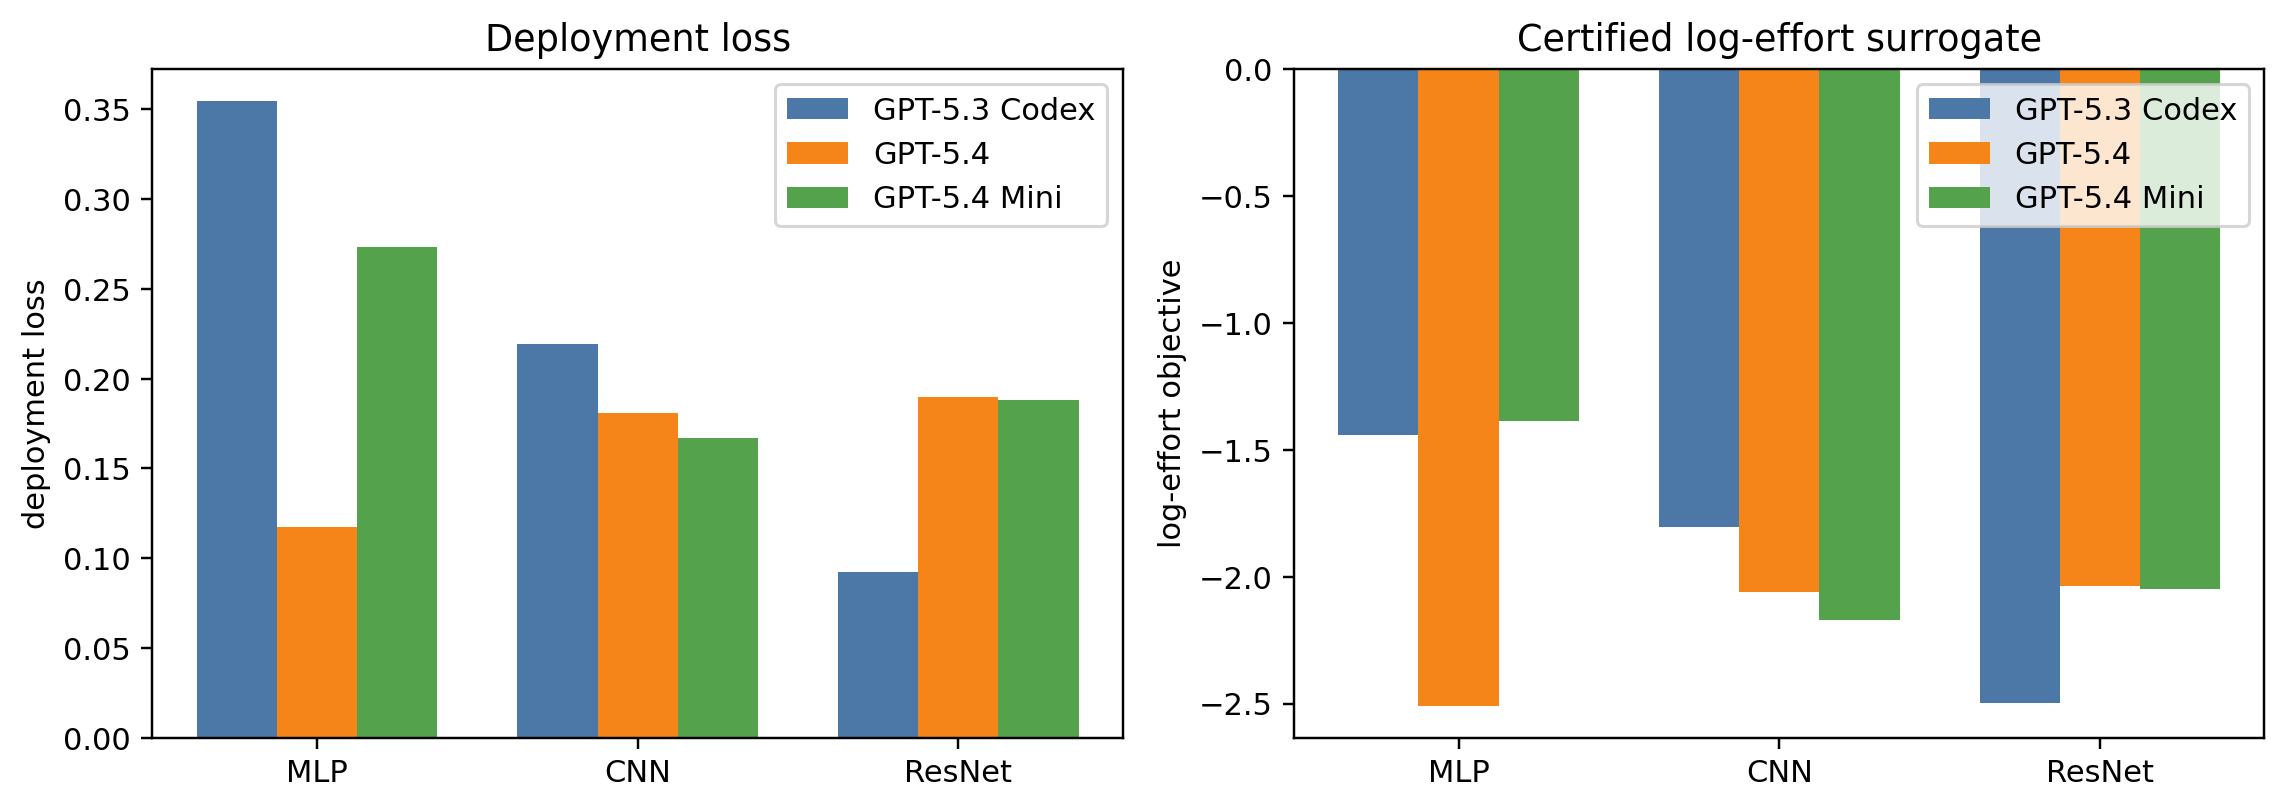
\includegraphics[width=\linewidth]{figures/autoresearch/threeworker_deployment_frontier.png}
\caption{Worker-frontier visualization for the accounting quantities in Table~\ref{tab:worker-frontier-accounting}.
\oldtext{The plot is diagnostic only: the main text table reports the numerical terms used for the deployment recommendation.}
\newtext{The plot is diagnostic only: the main text table reports the numerical terms used for the finite-horizon certified-time audit.}}
\label{fig:app-threeworker-frontier}
\end{figure}

\begin{figure}[ht]
\centering
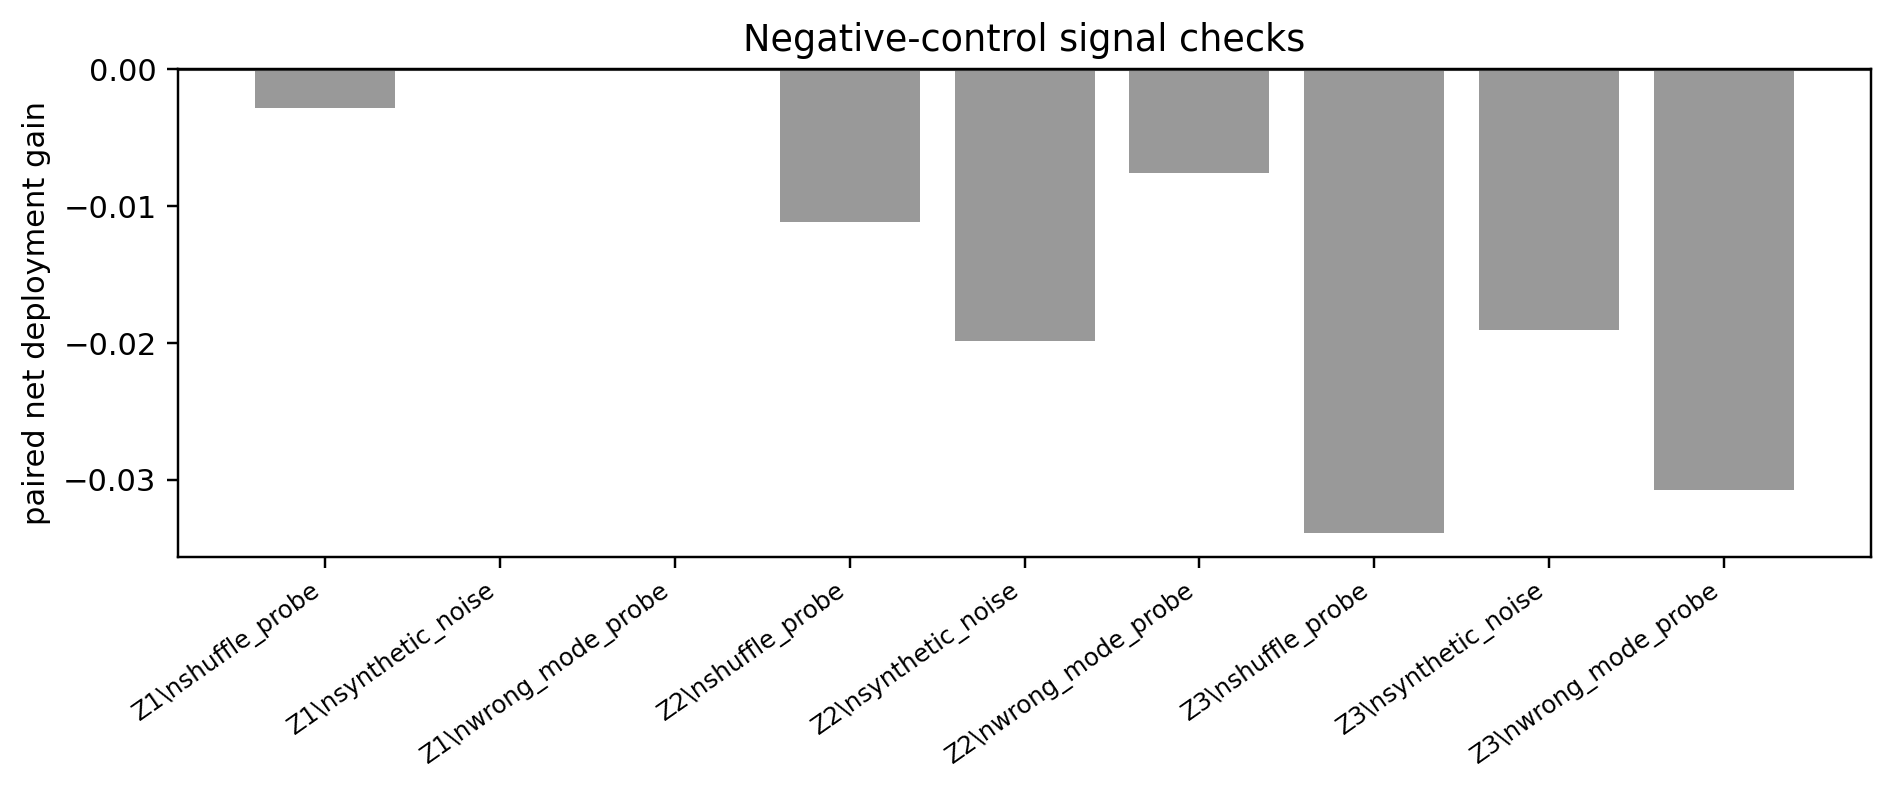
\includegraphics[width=\linewidth]{figures/autoresearch/threeworker_negative_controls.png}
\caption{Earlier probe-router negative-control audit for shuffled probes, wrong-mode probes, and synthetic noise records.
This diagnostic checks schema and context-burden artifacts for the probe-style router records; it is separate from the candidate-agent scout audit in Table~\ref{tab:candidate-scout-router}.}
\label{fig:app-negative-controls}
\end{figure}

\subsection{Pooled threshold and trajectory diagnostics}
\label{app:pilot-threshold-diagnostics}

\begin{figure}[p]
\centering
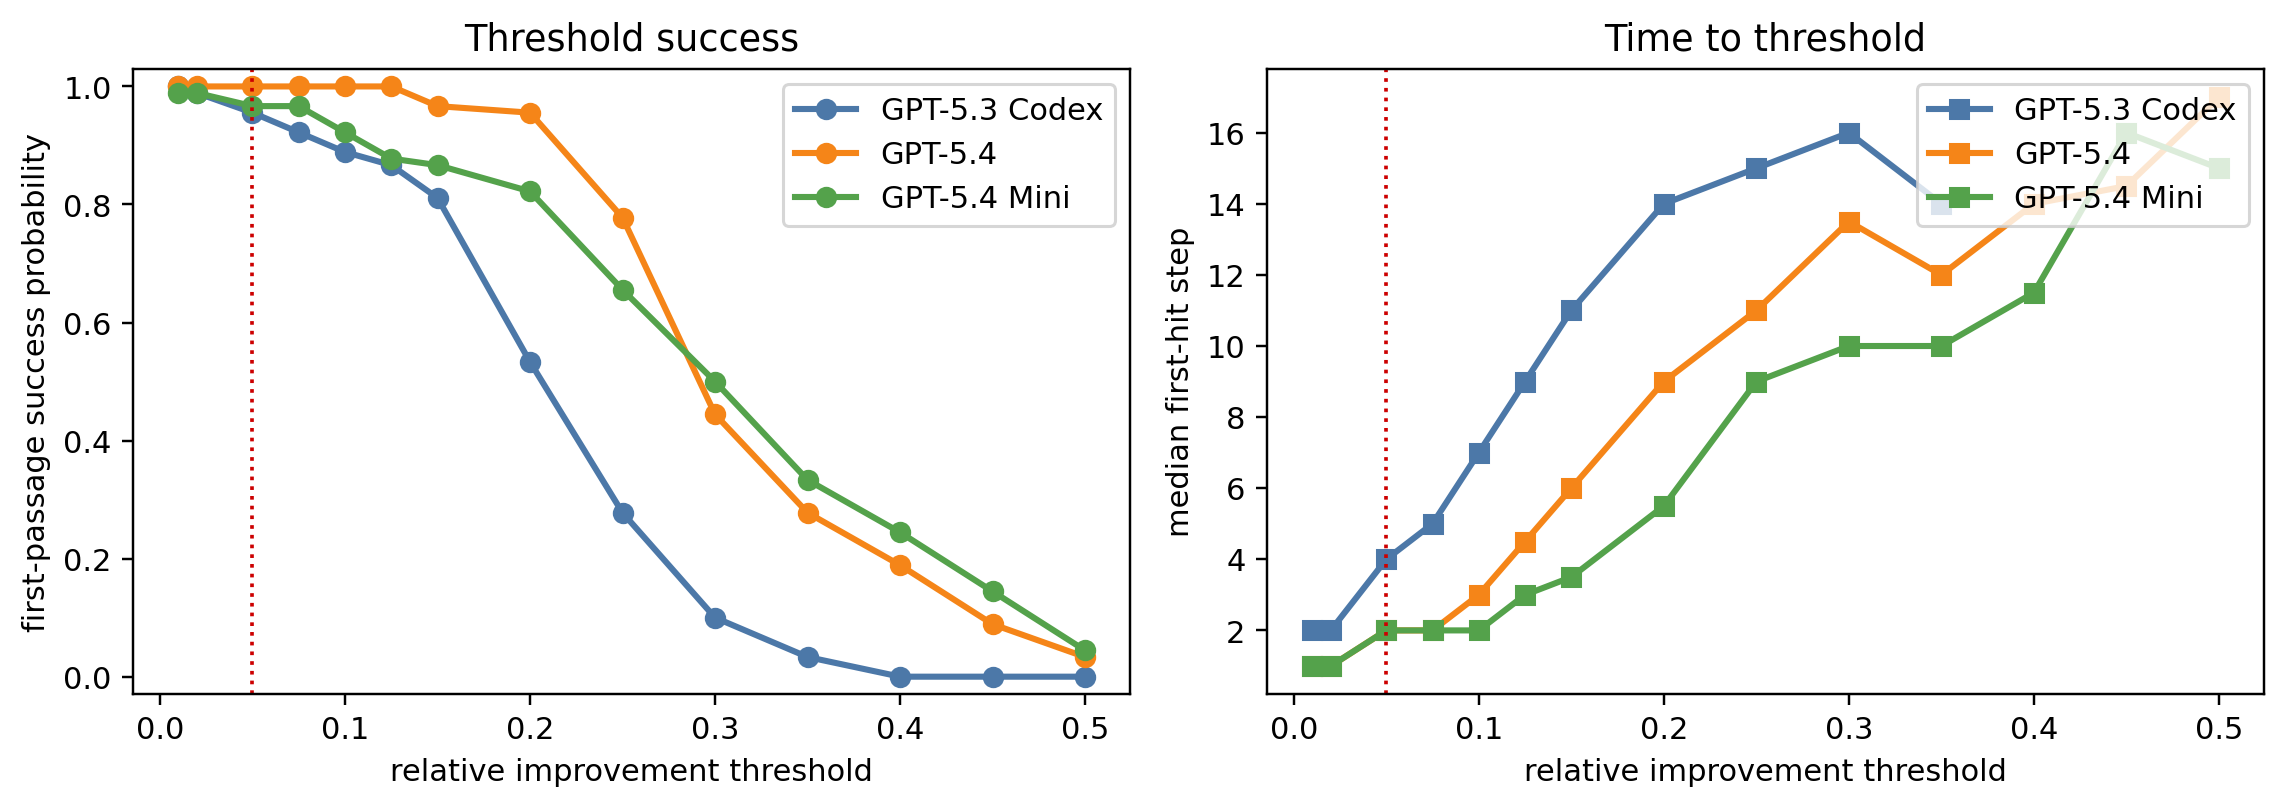
\includegraphics[width=\linewidth]{figures/autoresearch/threeworker_threshold_sensitivity.png}
\caption{Threshold sensitivity for the three-worker pooled panel.
The red line marks the operating threshold \(\gamma=0.05\).
At this threshold, entry success is near saturated while mean first-hit time remains low, which makes \(\gamma=0.05\) a pragmatic operating point for studying time-to-certified-solution.
The sharp drop at larger thresholds shows why the exact threshold is not an innocuous plotting choice.}
\label{fig:app-threshold-sensitivity-zoom}
\end{figure}

\begin{figure}[p]
\centering
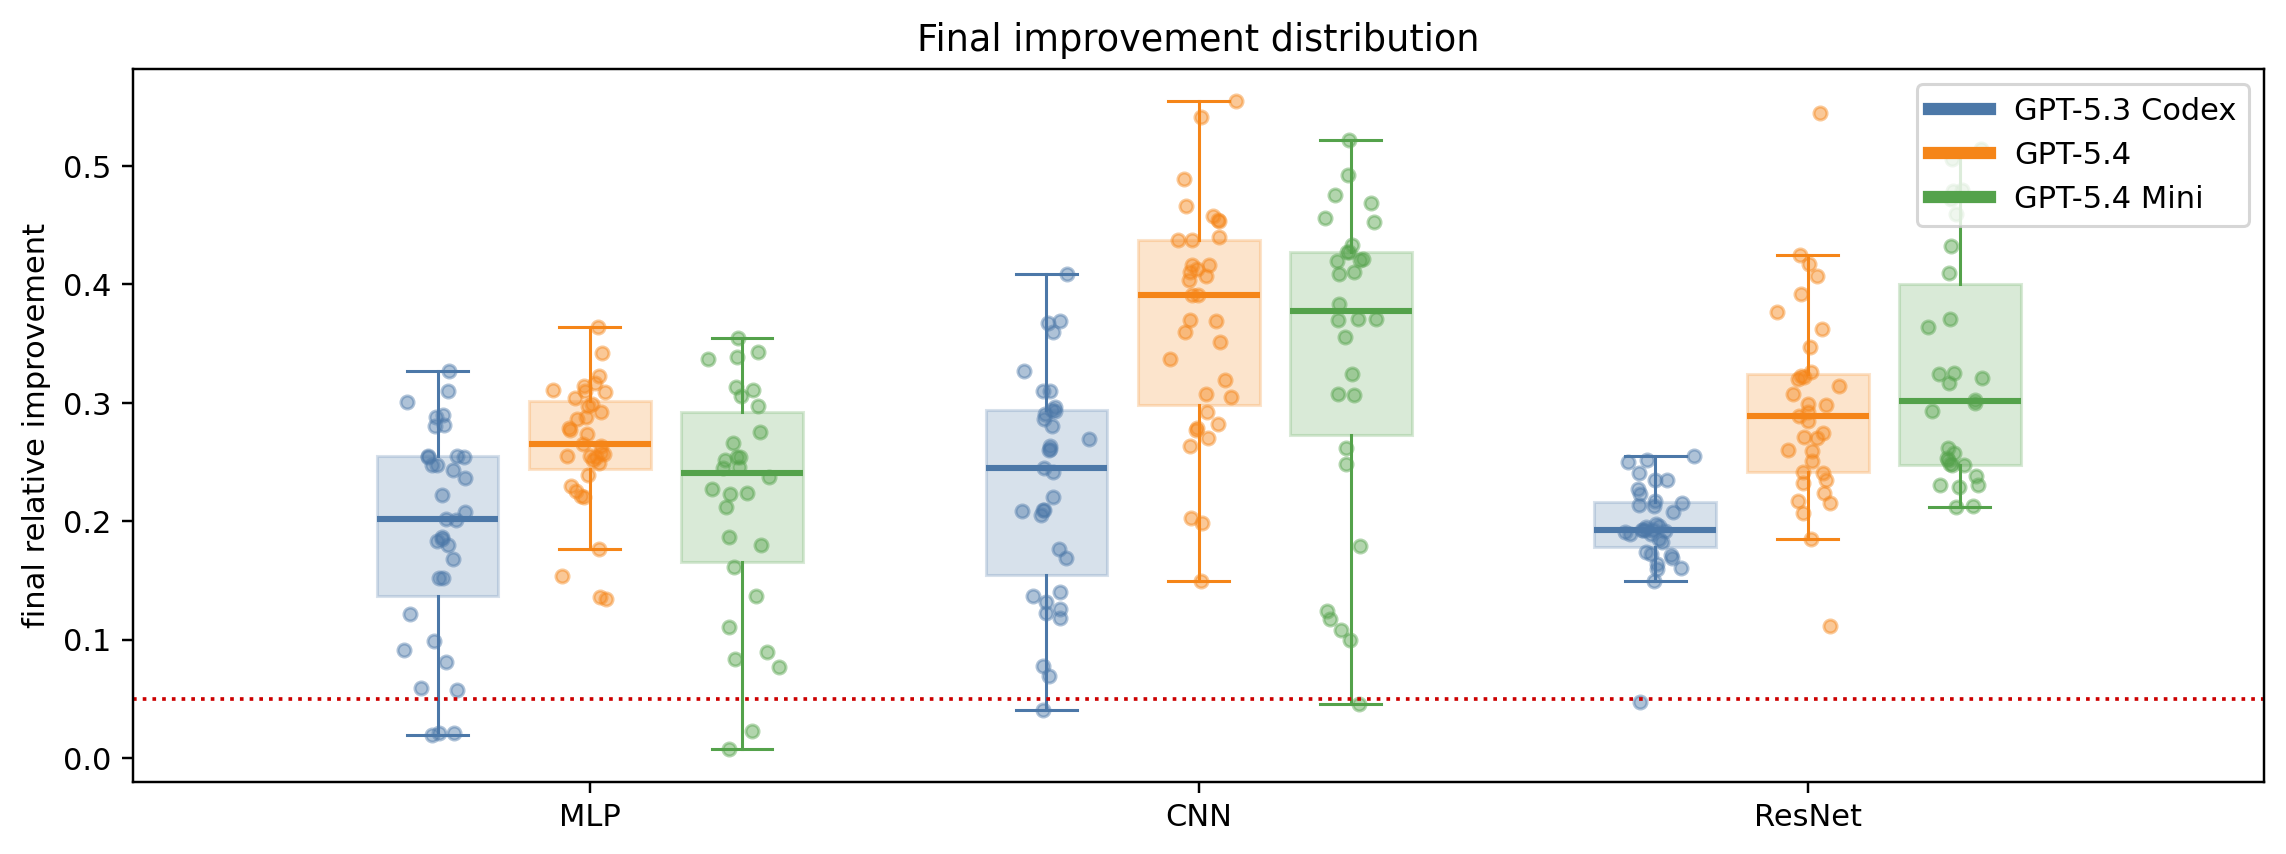
\includegraphics[width=\linewidth]{figures/autoresearch/threeworker_improvement_distribution.png}
\caption{Run-level improvement distribution for the three analyzed workers.
Dots show final best-visible relative improvement and thick ticks mark worker medians.
The survival plot makes the threshold choice explicit: near \(\gamma=0.05\), most runs succeed, but the ordering and separation change at higher thresholds.
\oldtext{This diagnostic supports the paper's claim that final quality, first-passage success, and deployment loss are distinct empirical objects.}
\newtext{This diagnostic supports the paper's claim that final quality, first-passage success, and certified time-to-threshold are distinct empirical objects.}}
\label{fig:app-improvement-distribution}
\end{figure}

\begin{figure}[p]
\centering
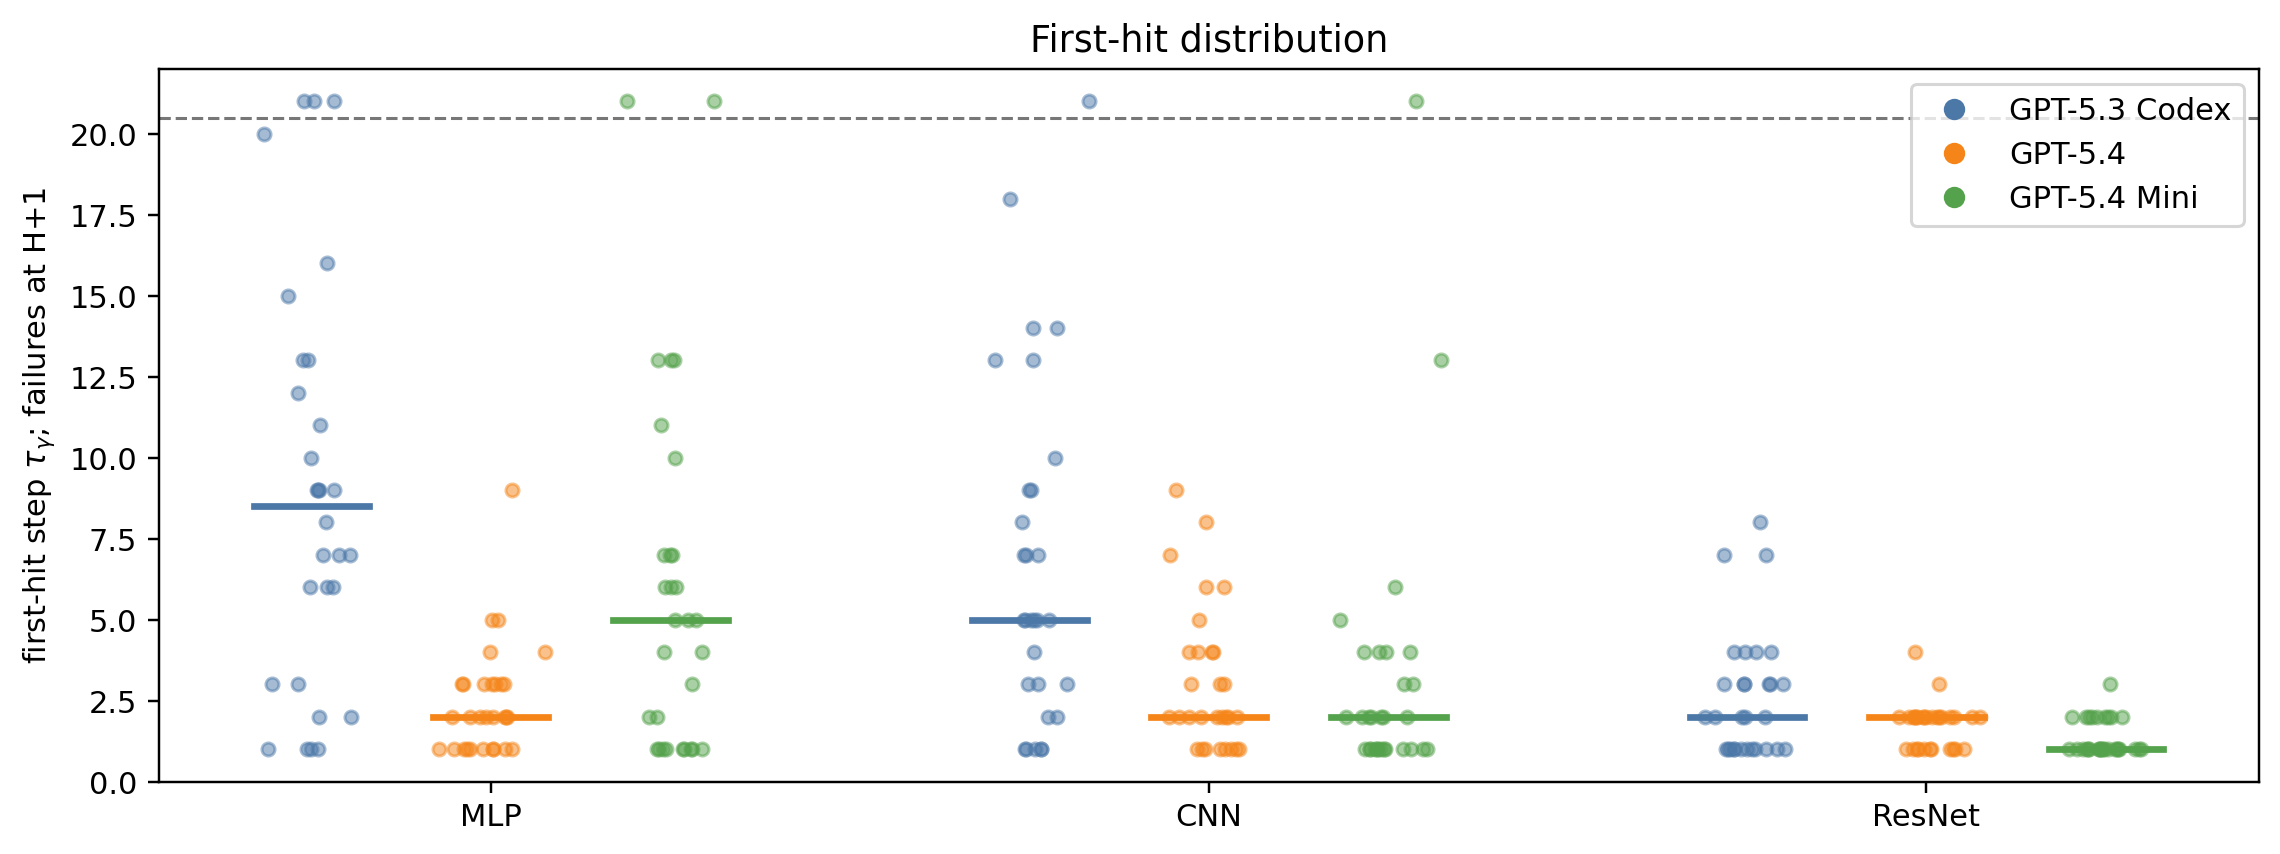
\includegraphics[width=\linewidth]{figures/autoresearch/threeworker_tau_distribution.png}
\caption{Pooled time-to-success distribution by task mode and worker.
The scatter plots expose mode-conditional heterogeneity: GPT-5.4 Mini is fastest on \textit{compact CNN} and \textit{micro ResNet}, while GPT-5.4 is fastest on \textit{MLP-flat}.
This is the empirical object behind the cost and competence terms of the four-term decomposition.}
\label{fig:app-tau-distribution}
\end{figure}

\begin{figure}[p]
\centering
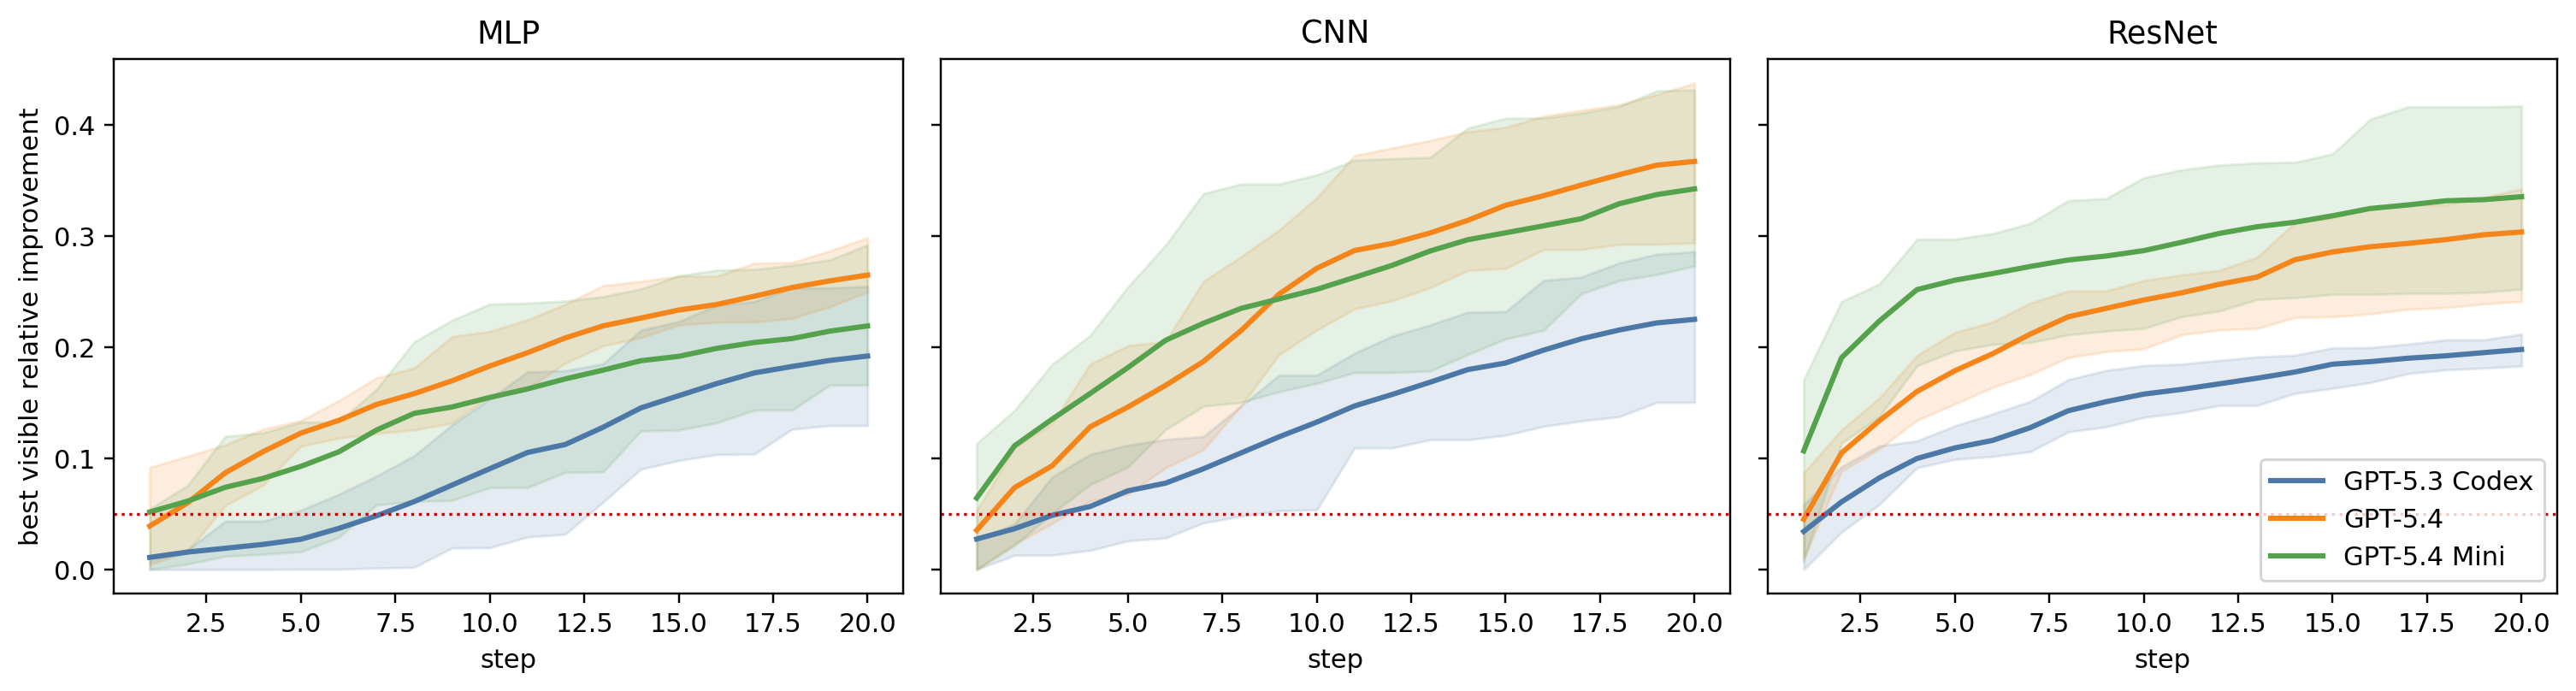
\includegraphics[width=\linewidth]{figures/autoresearch/threeworker_relative_improvement_trajectories.png}
\caption{Best-so-far improvement trajectories.
The mean trajectories show that early progress and final quality vary by mode and worker, but certified-time accounting in the main text shows that this does not automatically imply lower time-to-threshold after cost is charged.
This contrast is the main empirical reason to separate worker competence from certified-time value.}
\label{fig:app-improvement-trajectories}
\end{figure}

\subsection{Pooled cost diagnostics}
\label{app:pilot-cost-diagnostics}

\begin{figure}[p]
\centering
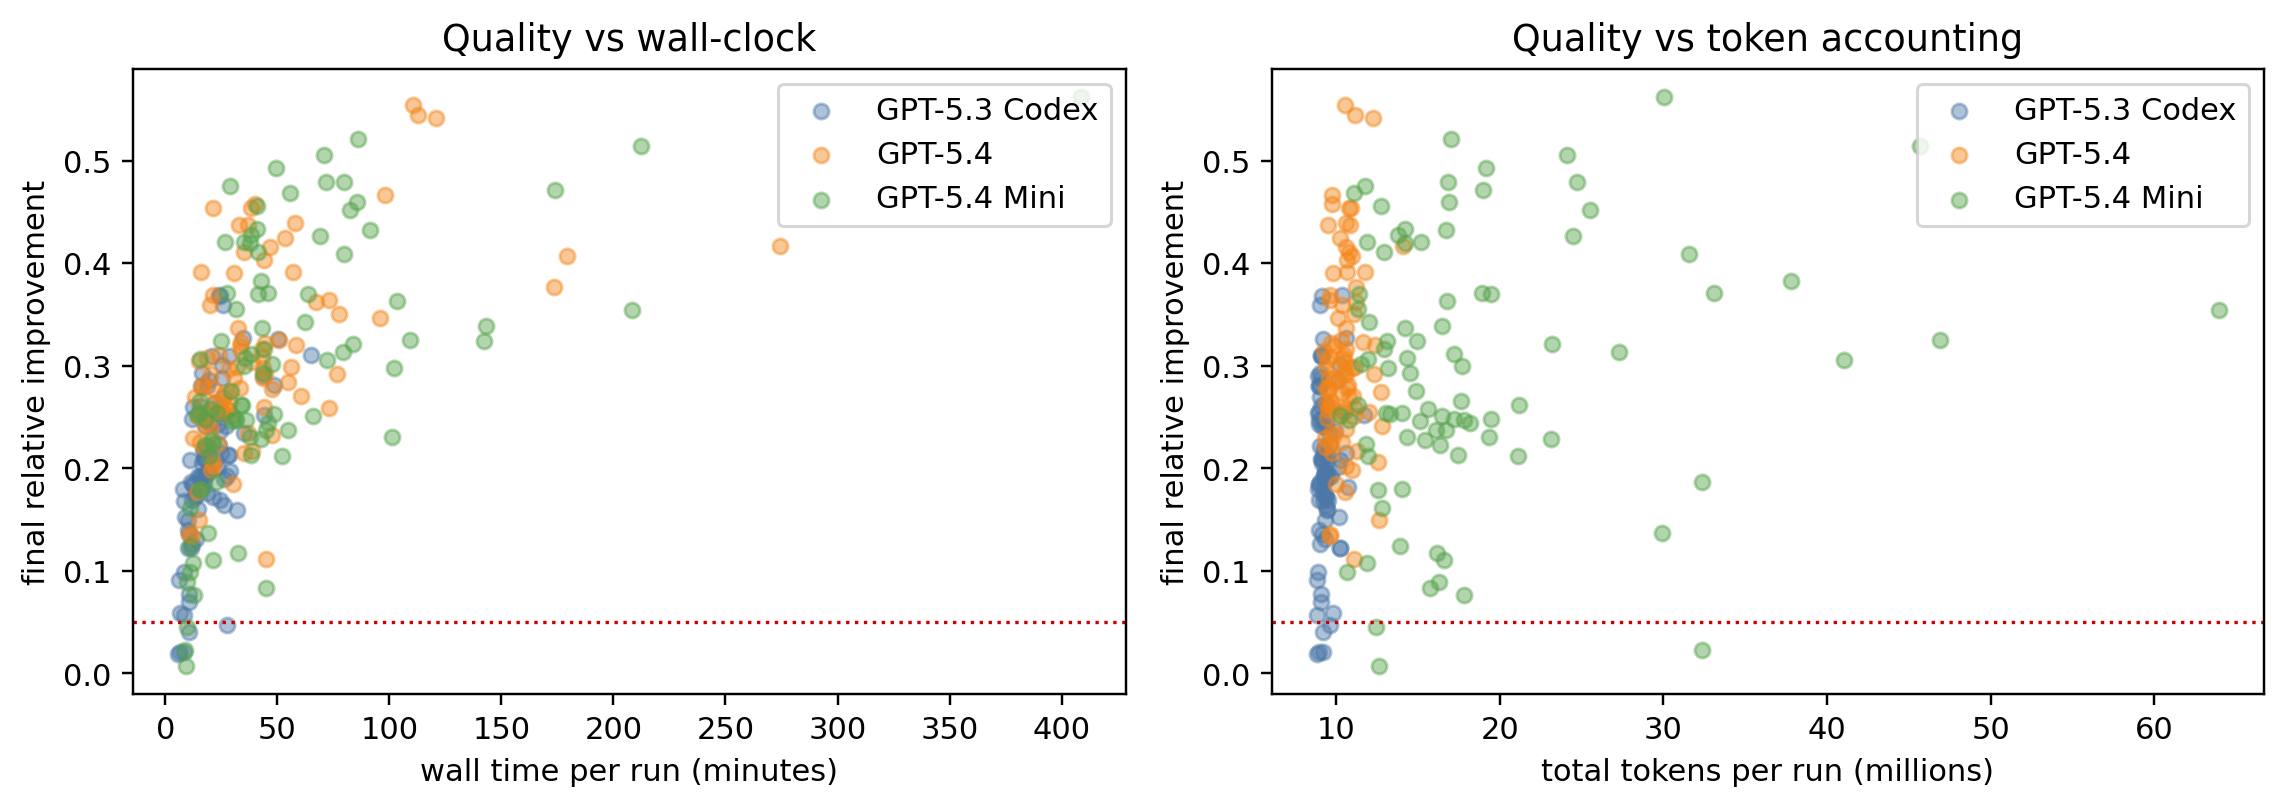
\includegraphics[width=\linewidth]{figures/autoresearch/threeworker_worker_cost_quality_diagnostics.png}
\caption{Worker cost--quality diagnostics.
Each point is a valid pooled run.
The plots show that better final improvement is accompanied by substantial variation in wall-clock time, total token accounting, and generated-token volume.
This supports the paper's budget-aware framing: worker choice cannot be reduced to final improvement alone.}
\label{fig:app-worker-cost-quality-full}
\end{figure}

\begin{figure}[p]
\centering
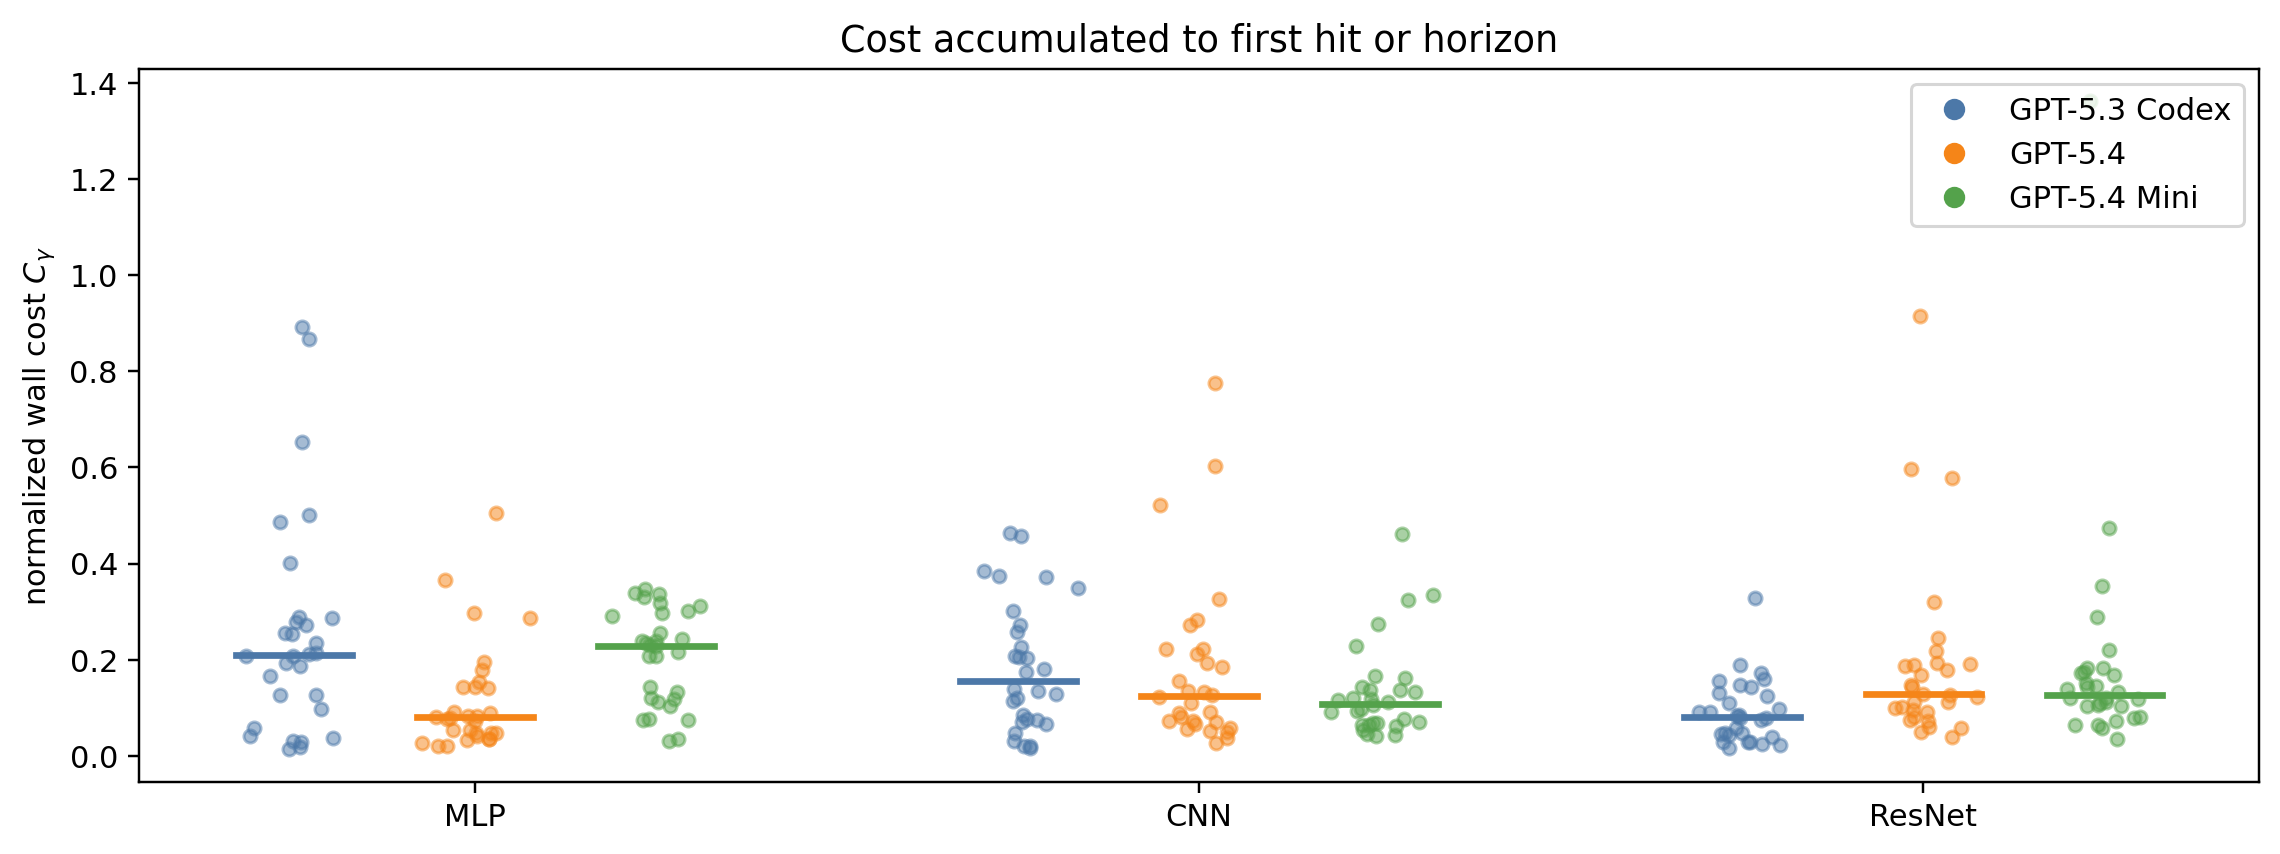
\includegraphics[width=\linewidth]{figures/autoresearch/threeworker_cost_to_tau_by_mode_worker.png}
\caption{Resource cost accumulated to first hit or horizon.
Mode-conditional cost spreads are large, which is why the retry-crossover theorem is treated as a cost-sensitive design rule rather than a generic endorsement of weaker workers.}
\label{fig:app-cost-to-tau-full}
\end{figure}

\begin{figure}[p]
\centering
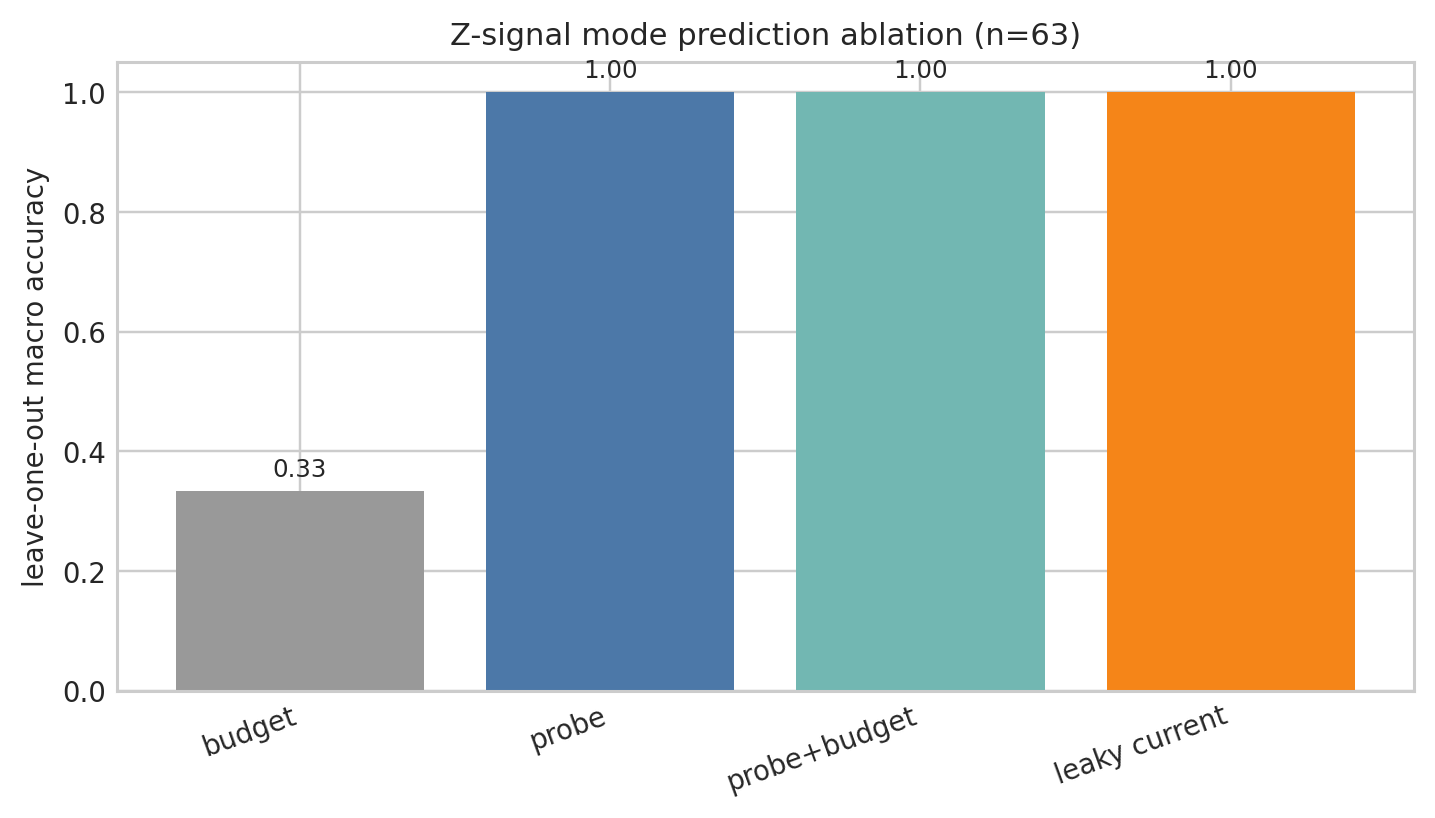
\includegraphics[width=0.92\linewidth]{figures/autoresearch/diag_z_signal_ablation.png}
\caption{Router-facing signal ablation.
The diagnostic tests whether progressively richer records expose the task-mode structure used in the accounting analysis.}
\label{fig:app-router}
\end{figure}

\clearpage
\section*{NeurIPS Paper Checklist}


\begin{enumerate}

\item {\bf Claims}
    \item[] Question: Do the main claims made in the abstract and introduction accurately reflect the paper's contributions and scope?
    \item[] Answer: \answerYes{}
    \item[] Justification: The abstract and introduction state the paper's scope: verifiable agentic systems, a packed latent-mode assumption, decomposition-guided selection, and a controlled fixed-prototype experimental protocol. The discussion section separates theory-facing and deployment-facing claims.
\item {\bf Limitations}
    \item[] Question: Does the paper discuss the limitations of the work performed by the authors?
    \item[] Answer: \answerYes{}
    \item[] Justification: Section~\ref{sec:discussion} discusses the packed-mode assumption, small live-agent sample sizes, finite design menus, oracle mode labels, and current cost-measurement limitations.
\item {\bf Theory assumptions and proofs}
    \item[] Question: For each theoretical result, does the paper provide the full set of assumptions and a complete (and correct) proof?
    \item[] Answer: \answerYes{}
    \item[] Justification: Assumption~\ref{ass:packed} states the assumptions for the main theoretical result, Theorem~\ref{thm:four-term} includes a proof sketch, and Appendix~\ref{app:proofs} gives the algebraic proof and pilot concentration details.
    \item {\bf Experimental result reproducibility}
    \item[] Question: Does the paper fully disclose all the information needed to reproduce the main experimental results of the paper to the extent that it affects the main claims and/or conclusions of the paper (regardless of whether the code and data are provided or not)?
    \item[] Answer: \answerYes{}
    \item[] Justification: Section~\ref{sec:experiments} describes the AutoResearch task instantiation, task modes, model menu, router-visible signals, horizons, metrics, and evaluation protocol; Appendix~\ref{app:experiment-details} specifies the required logs, estimators, and run-metadata fields.

\item {\bf Open access to data and code}
    \item[] Question: Does the paper provide open access to the data and code, with sufficient instructions to faithfully reproduce the main experimental results, as described in supplemental material?
    \item[] Answer: \answerNo{}
    \item[] Justification: The paper is written against an existing repository and includes reproducibility commands, but an anonymized public code/data release is not included in the current submission package.

\item {\bf Experimental setting/details}
    \item[] Question: Does the paper specify all the training and test details (e.g., data splits, hyperparameters, how they were chosen, type of optimizer) necessary to understand the results?
    \item[] Answer: \answerYes{}
    \item[] Justification: Section~\ref{sec:experiments} describes the AutoResearch task instantiation, task modes, model menu, router-visible signals, primary estimators, horizons, and evaluation design. Additional implementation details are listed in Appendix~\ref{app:experiment-details}.
\item {\bf Experiment statistical significance}
    \item[] Question: Does the paper report error bars suitably and correctly defined or other appropriate information about the statistical significance of the experiments?
    \item[] Answer: \answerYes{}
    \item[] Justification: Section~\ref{sec:experiments} and Appendix~\ref{app:experiment-details} specify Wilson intervals, bootstrap intervals, survival curves, calibration diagnostics, and held-out evaluation for the reported protocol.
\item {\bf Experiments compute resources}
    \item[] Question: For each experiment, does the paper provide sufficient information on the computer resources (type of compute workers, memory, time of execution) needed to reproduce the experiments?
    \item[] Answer: \answerNo{}
    \item[] Justification: The paper reports wall-clock costs and run counts but does not provide a complete compute-resource table for every experiment.
\item {\bf Code of ethics}
    \item[] Question: Does the research conducted in the paper conform, in every respect, with the NeurIPS Code of Ethics \url{https://neurips.cc/public/EthicsGuidelines}?
    \item[] Answer: \answerYes{}
    \item[] Justification: The work studies verifiable benchmark tasks and does not involve human subjects, sensitive personal data, or released high-risk models. The submission preserves anonymity and follows NeurIPS code and data policies.

\item {\bf Broader impacts}
    \item[] Question: Does the paper discuss both potential positive societal impacts and negative societal impacts of the work performed?
    \item[] Answer: \answerYes{}
    \item[] Justification: Section~\ref{sec:discussion} notes positive uses in cost-aware and transparent agent deployment as well as limitations and failure modes. The work is methodological and does not introduce a new generative model or dataset of people.
\item {\bf Safeguards}
    \item[] Question: Does the paper describe safeguards that have been put in place for responsible release of data or models that have a high risk for misuse (e.g., pre-trained language models, image generators, or scraped datasets)?
    \item[] Answer: \answerNA{}
    \item[] Justification: The paper does not release a pre-trained model, image generator, scraped dataset, or other asset with high misuse risk. It evaluates agent harnesses on synthetic or generated benchmark tasks.
\item {\bf Licenses for existing assets}
    \item[] Question: Are the creators or original owners of assets (e.g., code, data, models), used in the paper, properly credited and are the license and terms of use explicitly mentioned and properly respected?
    \item[] Answer: \answerYes{}
    \item[] Justification: The related-work section cites existing papers and systems used for positioning, and the experimental section describes the benchmark surfaces. Released code and benchmark assets include explicit license details.
\item {\bf New assets}
    \item[] Question: Are new assets introduced in the paper well documented and is the documentation provided alongside the assets?
    \item[] Answer: \answerYes{}
    \item[] Justification: The work introduces a code harness and analysis artifacts as research assets, and Appendix~\ref{app:experiment-details} documents the required logging and configuration fields.
\item {\bf Crowdsourcing and research with human subjects}
    \item[] Question: For crowdsourcing experiments and research with human subjects, does the paper include the full text of instructions given to participants and screenshots, if applicable, as well as details about compensation (if any)?
    \item[] Answer: \answerNA{}
    \item[] Justification: The paper does not involve crowdsourcing or research with human subjects.
\item {\bf Institutional review board (IRB) approvals or equivalent for research with human subjects}
    \item[] Question: Does the paper describe potential risks incurred by study participants, whether such risks were disclosed to the subjects, and whether Institutional Review Board (IRB) approvals (or an equivalent approval/review based on the requirements of your country or institution) were obtained?
    \item[] Answer: \answerNA{}
    \item[] Justification: The paper does not involve crowdsourcing or research with human subjects, so IRB or equivalent approval is not applicable.
\item {\bf Declaration of LLM usage}
    \item[] Question: Does the paper describe the usage of LLMs if it is an important, original, or non-standard component of the core methods in this research? Note that if the LLM is used only for writing, editing, or formatting purposes and does \emph{not} impact the core methodology, scientific rigor, or originality of the research, declaration is not required.
    %this research?
    \item[] Answer: \answerYes{}
    \item[] Justification: LLMs are central to the evaluated agent designs. Section~\ref{sec:experiments} describes the three-worker menu, fixed prompt-only router, sequential signal protocol, model-identifier logging, and routing-output requirements.
\end{enumerate}


\end{document}
